%% ----------------------------------------------------------------
%% main.tex --
%% ---------------------------------------------------------------- 

% Set up the document

%input includes
\documentclass[a4paper, 11pt, oneside]{Thesis}  % Use the "Thesis" style, based on the ECS Thesis style by Steve Gunn

\usepackage[T1]{fontenc} % Codificación de las fuentes utilizadas
\usepackage[spanish]{babel} % Español como idioma principal del texto (permite hyphenation de palabras al final de una línea)


\usepackage{graphicx}
\usepackage{url}

\graphicspath{{Figures/}{Diagrams}{Chapters/}}  % Location of the graphics files (set up for graphics to be in PDF format)

\selectlanguage{spanish}

\setcounter{tocdepth}{1}

% Include any extra LaTeX packages required
\usepackage[square, numbers, comma, sort&compress]{natbib}  % Use the "Natbib" style for the references in the Bibliography
\usepackage{verbatim}  % Needed for the "comment" environment to make LaTeX comments
\usepackage{vector}  % Allows "\bvec{}" and "\buvec{}" for "blackboard" style bold vectors in maths
\hypersetup{urlcolor=blue, colorlinks=true}  % Colours hyperlinks in blue, but this can be distracting if there are many links.
\usepackage{hyperref}
% \usepackage[pdfauthor={Diego Martín Arroyo},
%             pdftitle={Diseño e implementación de un sistema de computación distribuida con
% Raspberry Pi, y estudio comparativo del mismo frente a otras soluciones},
%             pdfsubject={Memora del Trabajo de Fin de Grado},
%             pdfproducer={XeLaTeX with hyperref},
%             pdfcreator={XeLaTeX},
%             pdfkeywords={Computación Paralela, Sistema Distribuido, Raspberry}
%             ]{hyperref}
%% ----------------------------------------------------------------

%% --------------------------------------------------------------------------------------------------------------------------------
%http://tex.stackexchange.com/a/85218/76599
\usepackage{fancyvrb}
\usepackage[dvipsnames]{xcolor}

% redefine \VerbatimInput
\RecustomVerbatimCommand{\VerbatimInput}{VerbatimInput}% Inclusión de archivos de texto plano
{fontsize=\footnotesize,
 %
 frame=lines,  % top and bottom rule only
 framesep=2em, % separation between frame and text
 rulecolor=\color{Gray},
 %
 label=\fbox{\color{Black}data.txt},
 labelposition=topline,
 %
 commandchars=\|\(\), % escape character and argument delimiters for
                      % commands within the verbatim
 commentchar=*        % comment character
}

\usepackage{listings} % Requerido para la inserción de código
%Listings command

\usepackage{float}
\newcommand*\lstinputpath[1]{\lstset{inputpath=#1}}
\lstinputpath{Code/}

\newcounter{undefinedreferences}
\setcounter{undefinedreferences}{0}

\newcommand{\citationneeded}[1][None]{\stepcounter{undefinedreferences}\textsuperscript{\color{blue} [Citation needed: #1]}}

\newcommand{\checkreferences}{
	\ifnum\value{undefinedreferences} > 0
	\begin{center}
		\immediate\write18{wget -O Figures/protester.png -nc http://imgs.xkcd.com/comics/wikipedian_protester.png}
		\includegraphics[width=\textwidth]{protester.png}\\
		There are \arabic{undefinedreferences} undefined references
	\end{center}
	\else
	No undefined references. Good!
	\fi
}


%https://github.com/pads-fhs/LaTeX-Template-Thesis/blob/master/lststyles.tex
\lstdefinelanguage{JavaScript}{
  keywords={typeof, new, true, false, catch,%
    function, return, null, catch, switch, var,%
    if, in, while, do, else, case, break},
  ndkeywords={class, export, boolean, throw, implements, import, this},
  sensitive=false,
  comment=[l]{//},
  morecomment=[s]{/*}{*/},
  morestring=[b]',
  morestring=[b]"
}
\newcommand{\lstsetjavascript}{
  \lstset{
		language=JavaScript,
		breaklines=true,
		commentstyle=\textit,
		basicstyle=\ttfamily,
		keywordstyle=\bfseries,
		stringstyle=\ttfamily,
		showstringspaces=false,
		frame=single,
		tabsize=2
  }
}

\lstdefinelanguage{log}{
  keywords={typeof, new, true, false, catch,%
    function, return, null, catch, switch, var,%
    if, in, while, do, else, case, break},
  ndkeywords={class, export, boolean, throw, implements, import, this},
  sensitive=false,
  comment=[l]{//},
  morecomment=[s]{/*}{*/},
  morestring=[b]',
  morestring=[b]"
}
\newcommand{\lstsetlog}{
  \lstset{
		language=log,
		breaklines=true,
		commentstyle=\textit,
		basicstyle=\ttfamily,
		keywordstyle=\bfseries,
		stringstyle=\ttfamily,
		showstringspaces=false,
		frame=single,
		tabsize=2
  }
}

\lstloadlanguages{Java,XML, JavaScript, log}

\newcommand{\javascriptcode}[4]{
	\lstinputlisting[caption=#2,label=#1, firstline=#3, lastline=#4]{#1.json}
}

\newcommand{\logcode}[4]{
	\lstinputlisting[caption=#2,label=#1, firstline=#3, lastline=#4]{#1.log}
}

\usepackage[bottom]{footmisc} %The footnotes go at the bottom of t\usepackage{dtklogos}he page, instead next to the last line.
%Ajustes para Java
% \lstset{
% 	language=java,
%  	frame=single, % Un marco simple alrededor del código
%     basicstyle=\small\ttfamily, % Utilizar fuente true type pequeña
%     keywordstyle=[1]\color{Blue}\bf, % Funciones en negrita y azul
%     keywordstyle=[2]\color{Purple}, % Argumentos en morado
%     keywordstyle=[3]\color{Blue}\underbar, % Funciones personalizadas subrayadas en azul
%     identifierstyle=, % Nada especial acerca de identificadores
%     commentstyle=\usefont{T1}{pcr}{m}{sl}\color{Green}\small, % Los comentarios se renderizan en fuente pequeña verde
%     stringstyle=\color{Purple}, % Cadenas en morado
%     showstringspaces=false, % No se muestran los espacios entre cadenas
%     tabsize=5, % 5 espacios por tabulado
%     %
%     % Put standard Perl functions not included in the default language here
%     %morekeywords={rand},
%     %
%     % Put Perl function parameters here
%     %morekeywords=[2]{on, off, interp},
%     %
%     % Put user defined functions here
%     %morekeywords=[3]{test},\usepackage{dtklogos}
%    	%
%     morecomment=[l][\color{Blue}]{...}, % Line continuation (...) like blue comment
%     numbers=left, % Número de línea a la izquierda
%     firstnumber=1, % Número de línea comienza en 1
%     numberstyle=\tiny\color{Blue}, % Los números de línea son azules y pequeños
%     stepnumber=5, % Los números de línea van de 5 en 5
%     breaklines=true % Salto de línea si el texto no entra. See http://stackoverflow.com/a/1875803
% }

%\usepackage{xltxtra} % XeLaTeX logo. Yep, just that
%http://tex.stackexchange.com/a/73179/76599
\usepackage{metalogo}
\usepackage{dtklogos} %BibTeX logo

%\usepackage{lscape}
\usepackage{pdflscape}
\begin{document}

\newcommand{\nombre}{Diseño e implementación de un sistema de computación distribuida con
Raspberry Pi, y estudio comparativo del mismo frente a otras soluciones}
\frontmatter      % Begin Roman style (i, ii, iii, iv...) page numbering


\newcommand{\autor}{Diego Martín Arroyo}

% Set up the Title Page
\title  {\nombre}
\authors  {\texorpdfstring
            {\href{tfg.martinarroyo.net}{Diego Martín Arroyo}}
            {Diego Martín Arroyo}
            }
\addresses  {\groupname\\\deptname\\\univname}  % Do not change this here, instead these must be set in the "Thesis.cls" file, please look through it instead
\date       {\today}
\subject    {}
\keywords   {}

\maketitle
%% ----------------------------------------------------------------

\setstretch{1.3}  % It is better to have smaller font and larger line spacing than the other way round

% Define the page headers using the FancyHdr package and set up for one-sided printing
\fancyhead{}  % Clears all page headers and footers
\rhead{\thepage}  % Sets the right side header to show the page number
\lhead{}  % Clears the left side page header

\pagestyle{fancy}  % Finally, use the "fancy" page style to implement the FancyHdr headers

%% ----------------------------------------------------------------
% Declaration Page required for the Thesis, your institution may give you a different text to place here
\Declaration{

\addtocontents{toc}{\vspace{1em}}  % Add a gap in the Contents, for aesthetics

Yo, \autor, declaro que la autoría de este Trabajo de Fin de Grado titulado, `\nombre' y el trabajo presentado en el mismo corresponde a mi persona. Confirmo que:

\begin{itemize} 
\item[\tiny{$\blacksquare$}] Este trabajo fue realizado completamente durante mis estudios del Grado en Ingeniería Informática en la Universidad de Salamanca.
 
\item[\tiny{$\blacksquare$}] En aquellas partes de este Trabajo que han sido previamente presentadas como Trabajo de Fin de Grado o cualquier otro tipo de disertación en esta Universidad u cualquier otra institución, esto ha sido claramente indicado.
 
\item[\tiny{$\blacksquare$}] Que todo el trabajo de terceros que ha sido consultado ha sido apropiadamente atribuido.

\item[\tiny{$\blacksquare$}] Donde haya citado el trabajo de otros, la fuente ha sido siempre dada. A excepción de dichas citas, todo el conjunto del Trabajo ha sido realizado por mí.
 
\item[\tiny{$\blacksquare$}] He reconocido todas aquellas fuentes de ayuda.
 
\item[\tiny{$\blacksquare$}] Donde mi Trabajo ha sido parte de una colaboración con otras personas, he indicado claramente la extensión de mi trabajo y el de dichos terceros.
\\
\end{itemize}
 
 
Firmado:\\
\rule[1em]{25em}{0.5pt}  % This prints a line for the signature
 
Fecha:\\
\rule[1em]{25em}{0.5pt}  % This prints a line to write the date
}
\clearpage  % Declaration ended, now start a new page

%% ----------------------------------------------------------------
\pagestyle{empty}  % No headers or footers for the following pages

\null\vfill
% Now comes the "Funny Quote", written in italics
Gather ye rosebuds while ye may,\\
Old Time is still a-flying:\\
And this same flower that smiles to-day\\
To-morrow will be dying.\\
 
The glorious lamp of heaven, the sun,\\
The higher he's a-getting,\\
The sooner will his race be run,\\
And nearer he 's to setting.\\
 
That age is best which is the first,\\
When youth and blood are warmer;\\
But being spent, the worse, and worst\\
Times still succeed the former.\\
 
Then be not coy, but use your time,\\
And while ye may, go marry:\\
For having lost but once your prime,\\
You may for ever tarry.\\

\begin{flushright}
Robert Herrick
\end{flushright}

\vfill\vfill\vfill\vfill\vfill\vfill\null
\clearpage  % Funny Quote page ended, start a new page
%% ----------------------------------------------------------------

% The Abstract Page
\addtotoc{Resumen}  % Add the "Abstract" page entry to the Contents
\abstract{
\addtocontents{toc}{\vspace{1em}}  % Add a gap in the Contents, for aesthetics

El uso de un sistema distribuido como alternativa a un equipo de altas prestaciones es una práctica aprovechada desde hace décadas en todo tipo de entornos. El auge de sistemas embebidos con gran potencia de cálculo y bajo coste en la actualidad ha motivado su utilización para la construcción de este tipo de sistemas de computación. Sin embargo, la mayoría de las soluciones responden a una necesidad específica. En el presente documento y los anexos que lo acompañan se plantea y desarrolla la creación de un sistema distribuido compuesto por placas Raspberry Pi que es aprovechable por un gran rango de usuarios con diferentes necesidades (investigadores, desarrolladores\dots), destacando su papel como herramienta didáctica. El resultado final consiste en un sistema escalable y autoconfigurado que incluye un amplio abanico de herramientas de desarrollo.

El desarrollo del sistema ha implicado la construcción de protocolos, utilidades y aplicaciones en diferentes capas, desde servicios provistos por el sistema operativo, pasando por utilidades consumibles por aplicaciones hasta aplicaciones que interactúan con usuarios finales. Todas estas adiciones son transparentes al usuario y altamente integrables con \textit{software} preexistente.

El proceso de desarrollo es precedido por una serie de etapas de evaluación y de un estudio de las diferentes alternativas valoradas antes de proceder a la construcción del sistema.

}

\clearpage  % Abstract ended, start a new page


%% ----------------------------------------------------------------

\setstretch{1.3}  % Reset the line-spacing to 1.3 for body text (if it has changed)

% The Acknowledgements page, for thanking everyone
\acknowledgements{
\addtocontents{toc}{\vspace{1em}}  % Add a gap in the Contents, for aesthetics

The acknowledgements and the people to thank go here, don't forget to include your project advisor\ldots

}
\clearpage  % End of the Acknowledgements
%% ----------------------------------------------------------------

\pagestyle{fancy}  %The page style headers have been "empty" all this time, now use the "fancy" headers as defined before to bring them back


%% ----------------------------------------------------------------
\lhead{\emph{Contents}}  % Set the left side page header to "Contents"
\tableofcontents  % Write out the Table of Contents

%% ----------------------------------------------------------------
\lhead{\emph{List of Figures}}  % Set the left side page header to "List if Figures"
\listoffigures  % Write out the List of Figures

%% ----------------------------------------------------------------
\lhead{\emph{List of Tables}}  % Set the left side page header to "List of Tables"
\listoftables  % Write out the List of Tables

%% ----------------------------------------------------------------
\setstretch{1.5}  % Set the line spacing to 1.5, this makes the following tables easier to read
\clearpage  % Start a new page
\lhead{\emph{Abbreviations}}  % Set the left side page header to "Abbreviations"
\listofsymbols{ll}  % Include a list of Abbreviations (a table of two columns)
{
% \textbf{Acronym} & \textbf{W}hat (it) \textbf{S}tands \textbf{F}or \\
\textbf{LAH} & \textbf{L}ist \textbf{A}bbreviations \textbf{H}ere \\

}

\include{constants}

% Begin the Dedication page

\setstretch{1.3}  % Return the line spacing back to 1.3

\pagestyle{empty}  % Page style needs to be empty for this page
\dedicatory{For/Dedicated to/To my\ldots}

\addtocontents{toc}{\vspace{2em}}  % Add a gap in the Contents, for aesthetics


%% ----------------------------------------------------------------
\mainmatter	  % Begin normal, numeric (1,2,3...) page numbering
\pagestyle{fancy}  % Return the page headers back to the "fancy" style

% Include the chapters of the thesis, as separate files
% Just uncomment the lines as you write the chapters
\lhead{\emph{Introducción}}
\chapter{Introducción}

\begin{cabstract}
En el que se resumen los objetivos a cumplir durante el desarrollo del proyecto y los resultados finales.
\end{cabstract}

Los límites físicos de los que adolecen los computadores en la actualidad \cite{seth:physical} hacen de la computación distribuida un recurso para incrementar de forma sencilla y económica el rendimiento total de un sistema. Sumado a estos beneficios, el auge de sistemas como teléfonos inteligentes o aplicaciones web ha potenciado el auge de diferentes paradigmas distribuidos en los últimos años. 

Sin embargo, estas ganancias conllevan una serie de inconvenientes entre los que figura el aumento de la complejidad del sistema. En general, un sistema distribuido requiere un conjunto de entidades independientes, más difíciles de configurar y mantener que una única entidad. Además, aparecen nuevos problemas: comunicación, integridad y sincronización, dificultad en el desarrollo y depuración de aplicaciones, etcétera.

En el apartado didáctico, el estudio del paradigma distribuido suele requerir un gran esfuerzo por parte de los estudiantes, en particular a la hora de comprender los fundamentos básicos de cualquier aplicación distribuida así como a la hora de realizar tareas de análisis y depuración.

Otro de los problemas que acompañan a la utilización de este tipo de sistemas reside en las comunicaciones entre nodos. Ejemplos de este tipo de problemas son la identificación de los diferentes componentes y sus propiedades o los canales de comunicación a establecer y su eficiencia y fiabilidad.

A dichas dificultades técnicas se suman otras de carácter económico o logístico. Generalmente el coste de estos equipos es elevado (si bien la relación coste/beneficio es muy atractiva) y presentan una serie de requisitos de espacio, instalación y mantenimiento difíciles de satisfacer por algunas organizaciones.

La presente memoria recoge el proceso de evaluación de diferentes alternativas para la creación de un sistema distribuido que define entre sus objetivos funcionales el carácter multipropósito, la autoconfiguración de los diferentes componentes y la reducción del coste total, utilizando equipos ya existentes en la organización donde se integrará o adquiriendo componentes económicos. Posteriormente se describirán las diferentes etapas de diseño y desarrollo de una propuesta de solución al problema: un sistema formado por dispositivos Raspberry Pi y un conjunto de protocolos, herramientas y servicios para la utilización del mismo como plataforma de investigación en el campo de la computación distribuida y como herramienta didáctica para disciplinas relacionadas con dicho área.

El sistema se compone de un conjunto de dispositivos físicos compuesto por los nodos de computación y una serie de módulos accesorios, así como los diferentes mecanismos de alimentación y refrigeración, un conjunto de paquetes \textit{software} que permiten la coordinación y comunicación entre los diferentes procesos y una serie de herramientas que facilitan el trabajo con el sistema.

Además, se incluyen las definiciones de los diferentes conceptos teóricos necesarios para la creación del sistema, así como las diferentes etapas de aprendizaje, análisis de alternativas y diferentes procesos de evaluación llevados a cabo durante las diferentes etapas desarrollo, así como las metodologías de trabajo utilizadas, sin olvidar la documentación de todas las herramientas creadas.

El producto final creado prueba que la utilización de sistemas embebidos de bajo coste, si bien limitados en rendimiento, constituyen una alternativa económica frente a soluciones como el empleo de equipos de escritorio o computadores diseñados de forma específica para este propósito.

\lhead{\emph{Motivación}}
\chapter{Motivación}

\section{Introducción}

Los límites físicos de los que adolecen los computadores en la época actual\citationneeded hacen de los paradigmas de Computación Distribuida y Paralela un recurso para incrementar de forma sencilla y económica el rendimiento total de un sistema, rendimiento que aumenta significativamente en problemas \textit{ridículamente paralelos}\citationneeded.

Sin embargo, estas ganancias conllevan una serie de inconvenientes, o el aumento de la complejidad de diversas tareas. En general, un sistema distribuido requiere un conjunto de máquinas independientes, que en conjunto suponen un coste superior al de un único nodo. Además, aparecen nuevos problemas de índole técnica: problemas de comunicación, integridad y sincronización, dificultad en el desarrollo y depuración de aplicaciones, etcétera.

En el apartado didáctico, el estudio del paradigma distribuido suele requerir un gran esfuerzo por parte de los estudiantes, en particular a la hora de comprender los fundamentos básicos de cualquier aplicación distribuida.

\section{Motivación y objetivos}

El sistema descrito en esta memoria surge inspirado en proyectos similares y las diferentes necesidades identificadas como estudiante del Grado en Ingeniería Informática. El Sistema se desarrolla con una serie de objetivos claros e independientes:

\begin{itemize}
	\item Como herramienta de síntesis de los conocimientos adquiridos en la carrera, se busca la creación de un sistema completo desde sus cimientos hasta los componentes de más alto nivel, gestionando las tareas de mantenimiento, instalación y manejo del mismo, así como los protocolos de trabajo, tanto en cada uno de los componentes del sistema como en la comunicación entre los mismos. Con un enfoque más teórico, se pretende crear un sistema capaz de poder ser utilizado como herramienta de diseño y prueba de algoritmos que resuelvan problemas aprovechando la distribución de tareas, así como el análisis de dichos algoritmos utilizando versiones finales del sistema.

	\item Potenciar el aprendizaje en las áreas de conocimiento Sistemas Operativos, Sistemas Embebidos, Redes de Computadores, Sistemas Distribuidos, Administración de Sistemas y Algoritmia.
	
	\item Constituir una herramienta didáctica para varias asignaturas cursadas en el plan de estudios del Grado en Ingeniería Informática en la Universidad de Salamanca, analizando las asignaturas de relevancia en el Plan y buscando soluciones a las necesidades propuestas por el Profesorado, Estudiantes y Administradores del sistema en colaboración con dichas partes.

	\item Intentar elevar el \textit{state of the art} en el mundo de los sistemas distribuidos con plataformas embebidas mediante la creación de un sistema multipropósito en lugar de soluciones con un fin determinado.

\end{itemize}

Partiendo de la premisa de las potenciales ventajas del uso de este tipo de computadores en detrimento de otras soluciones se plantea el sistema definitivo (ver \ref{alternativas}).

\section{Objetivos del sistema}

Durante las fases de definición del proyecto, se plantean los siguientes objetivos a cumplir para la consecución del sistema:

\subsection{Diseño y construcción de la arquitectura física del sistema}

Se deberán definir las interconexiones entre los diferentes componentes del sistema, solucionar los diferentes problemas físicos tales como la alimentación eléctrica, conexiones de red, refrigeración, entre otros, analizando los diferentes enfoques y valorando la mejor solución en función del resto de objetivos a cumplir.

\subsection{Gestión del sistema}

El sistema debe contar con un conjunto de herramientas que mantengan los principios de transparencia propios de un sistema distribuido\citationneeded.

\subsection{Integración}

El sistema debe integrarse en una infraestructura preexistente, sin que dicha integración comprometa el diseño básico del sistema, a fin de facilitar su adaptabilidad a otros entornos.

\subsection{Uso como herramienta didáctica}

El sistema debe ofrecer una serie de ventajas a las herramientas didácticas utilizadas en aquellas asignaturas donde se impartan conocimientos relacionados con la computación paralela y distribuida, ofreciendo herramientas que faciliten la comprensión de dichos paradigmas o el desarrollo, prueba y aplicación de programas basados en los mismos.

\subsection{Evaluación}

A fin de probar los objetivos definidos anteriormente, la viabilidad de sistema como herramienta didáctica y su integración en la organización deberán ser determinados por los diferentes usuarios de la misma.


Durante el desarrollo del proyecto se añaden los siguientes objetivos funcionales:

\subsection{Simplicidad de MarcoPolo}

MarcoPolo debe conseguir un alto grado de versatilidad y aplicabilidad en un gran rango de aplicaciones. A fin de conseguir este objetivo, la simplicidad del sistema construido es clave. Esto conlleva el desacoplamiento y delegación de gran parte de la funcionalidad a otras capas superiores, independientes del protocolo, pero que aprovechan su funcionalidad, en lugar de ser integradas en el mismo.

\subsection{Test-Driven Development}

El desarrollo de las diferentes herramientas \textit{software} se deberá realizar bajo los principios del desarrollo conducido por pruebas (ver \ref{tdd}) como mecanismo para la detección temprana de \textit{bugs}.

\section{Situación actual (\textit{state of the art})}

%Este apartado sería parecido a lo que en trabajos de grado (WHVLQDV \ WHVLV) se denomina estado del arte. En un proyecto de final de carrera de primer ciclo no parece obligada su presencia (D GLIHUHQFLD GHO VHJXQGR FLFOR GRQGH OD MXVWLILFDFLyQ WHyULFD PHGLDQWH XQ HVWDGR GHO DUWH GHEH DFRPSDxDU D ORV SURGXFWRV VRIWZDUH UHDOL]DGRV), aunque se puede dejar a juicio del tutor o tutores el incluir un pequeño resumen comentado de los trabajos y proyectos ya realizados en el campo del proyecto en curso.


\subsection{Computadores de placa única}

El uso de computadores de prestaciones reducidas como componentes de un sistema distribuido ha experimentado un gran crecimiento en los últimos años debido a la popularización y el abaratamiento de este tipo de dispositivos, existiendo gran cantidad de fabricantes y proveedores de \textit{software} para los mismos.

Los computadores de placa única (\textit{Single-Board Computer}) consisten en computadores de generalmente bajas prestaciones que aglutinan todos los componentes necesarios para su funcionamiento en un único circuito integrado. Dichas placas suelen tener un coste bajo y una relación rendimiento/coste muy elevada.

Durante los últimos años se han popularizado como una herramienta para el estudio y creación de sistemas distribuidos con un gran rango de propósitos diferentes.

\subsubsection{RPiCluster (Joshua Kiepert)}

Joshua Kiepert, estudiante de doctorado en la universidad Boise State, crea este sistema utilizando 33 computadores \textbf{Raspberry Pi B}, con el objetivo de utilizarlo como herramienta de pruebas que sirva de alternativa al supercomputador situado en su universidad\cite{joshuarpicluster}, sobre el que trabaja de forma rutinaria, a fin de poder continuar su trabajo en periodos de mantenimiento, cierre del centro, etcétera. El sistema está diseñado para utilizar la \textit{Message Passing Interface} como mecanismo de comunicación y coordinación (siguiendo un esquema maestro-esclavo) y además poder utilizar los diferentes puertos de las placas (GPIO, I\textsuperscript{2}C, SPI, UART), puertos generalmente ausentes en computadores utilizados para este tipo de propósitos. Utiliza además un servidor \textbf{NFS} para compartir datos entre todos los nodos, y un \textit{router} dedicado para la interconexión. El sistema se complementa con un ordenador \textbf{Chromebook} con el mismo sistema operativo (\textbf{Arch Linux}), que actúa como nodo coordinador.

Está compuesto del conjunto de nodos esclavos y coordinador, dos fuentes de alimentación y un mecanismo de refrigeración. El sistema cuenta con su propio mecanismo de distribución de la energía (diseñado por Kiepert) y de gestión de los LEDs. 

% http://www.zdnet.com/article/build-your-own-supercomputer-out-of-raspberry-pi-boards/

\begin{figure}[H]
\centering
\includegraphics[width=0.4\textwidth]{Chapter1/Figures/kiepert-main}
\includegraphics[width=0.4\textwidth]{Chapter1/Figures/structure.png}
\caption{Vista general y estructura del sistema (Fuente: Joshua Kiepert)}
\label{kiepert:structure}
\end{figure}

\textbf{Coste}: 1967.21 dólares.

\subsubsection{Dramble (Jeff Geerling)}

El clúster \textit{Dramble} es un conjunto de 6 equipos \textbf{Raspberry Pi} capaces de ejecutar en conjunto el gestor de contenidos \textbf{Drupal}\footnote{\href{https://www.drupal.org/}{drupal.org}}. El sistema es utilizado como servidor de pruebas para la ejecución de instancias de este \textit{software} de forma experimental o durante demonstraciones en público\cite{geerlingraspberry}. Se compone del conjunto de nodos Rasbperry Pi y los mecanismos de red que interconectan los nodos.

\begin{figure}[H]
\centering
\includegraphics[width=0.5\textwidth]{Chapters/Chapter1/Figures/raspberry-pi-dramble-cluster-wired.jpg}
\caption{El \textit{Dramble} en ejecución}
\label{geerling:dramble}
\end{figure}

\textbf{Coste (estimado)}: 35 dólares por cada Raspberry Pi mas el coste añadido de la red.

\subsubsection{Bramble (GCHQ)}

El organismo gubernamental \textit{Government Communication Headquarters}, agencia de inteligencia del Gobierno Británico presentó en la \textit{Big Bang Fair} de 2015 un proyecto educativo que combina 66 \textit{Raspberry Pi} en un clúster jerárquico con 8 grupos de 8 nodos, cada uno de ellos con un coordinador interno. El cableado se reduce gracias al uso de la tecnología \textbf{PoE} (\textit{Power over Ethernet}), y cada \textbf{Raspberr} cuenta con un conjunto de elementos adicionales, como un reloj de tiempo real, disco duro externo, cámara, o punto de acceso WiFi\cite{gchqbramble}.

\begin{figure}[H]
\centering
\includegraphics[width=0.5\textwidth]{Chapters/Chapter1/Figures/bramblegchq}
\caption{Vistazo general de la estructura del sistema}
\label{gchq:bramble}

\textbf{Coste} Se desconocen datos sobre el coste total del sistema.

\end{figure}

\subsubsection{Clúster Iridis (Simon Cox, University of Southampton)}

Con el objetivo de atraer a jóvenes estudiantes al mundo de la Computación, el profesor Simon Cox crea este clúster con 64 \textbf{Raspberry Pi B} sobre una estructura de LEGO\cite{cox:raspberry}.
\begin{figure}[H]
\centering
\includegraphics[width=0.5\textwidth]{Chapters/Chapter1/Figures/iridis-pi.jpg}
\caption{Sistema}
\label{cox:iridis}

\textbf{Coste} Se desconocen datos sobre el coste total del sistema

\end{figure}

\subsubsection{Paralella}

Paralella es un proyecto de la compañía Adapteva que integra en un único chip un conjunto elevado de procesadores independientes con el objetivo de incrementar la capacidad de procesamiento total del sistema a un coste muy reducido\cite{paralella}.

\textbf{Coste} 99 dólares por unidad. % Introduction

\lhead{\emph{Conceptos teóricos}}

\chapter{Conceptos teóricos}

\section{Programación orientada a eventos}
\label{eventdriven}

La programación orientada a eventos (\textit{event-driven programming}) constituye un patrón de programación en el cual el flujo del programa no se define íntegramente de forma secuencial, sino por las diversas interacciones (eventos) que el \textit{software} recibe durante su ejecución. Dichos eventos, generalmente imprevisibles, son causados por cualquier otra aplicación o entidad externa, y su naturaleza es muy variada: interacciones de ratón o teclado, conexiones de red o estímulos de sensores son claros ejemplos.

La programación orientada a eventos constituye un patrón exitoso en varios tipos de aplicaciones, en particular aplicaciones con interfaz gráfica de usuario o aplicaciones de un único hilo (\textit{single-threaded applications}). 

Si bien existen una gran cantidad de herramientas para el desarrollo de \textit{software} siguiendo este patrón, el funcionamiento de todas ellas se reduce a un conjunto de manejadores y disparadores de eventos. También reciben nombres similares, como señales y ranuras.

\subsection{Suscriptor de eventos}

Un suscriptor de eventos permite vincular un evento a un manejador. Por ejemplo:

\begin{lstlisting}
document.onmousemove=manejadorMouseMove
\end{lstlisting}

\subsection{Manejador de eventos}

Un manejador (\textit{handler}) determina la acción a realizar al recibir un evento. En una gran cantidad de \textit{frameworks} se definen como funciones.

\begin{lstlisting}
function manejadorMouseMove(evento){
	console.log(evento.pageX);
}
\end{lstlisting}

\section{Computación distribuida}

Un sistema distribuido es aquel conformado por un conjunto de nodos independientes que son percibidos como una entidad única y coherente por el usuario final. Dicha definición implica dos conceptos de importancia en el paradigma:

\begin{itemize}
  \item Autonomía: los diferentes integrantes del sistema cuentan con un alto grado de autonomía entre sí, y por tanto se deben diseñar e implementar mecanismos de comunicación entre los mismos, mecanismos que formarán parte del núcleo del sistema, y cuyo diseño tendrá consecuencias directas en el funcionamiento final del sistema.
  \item Transparencia: Las diferencias entre diferentes nodos suelen ser invisibles para los usuarios finales, así como la gestión de fallos y recuperación y la uniformidad a la hora de interactuar con el sistema. Según \citationneeded las siguientes propiedades del sistema deben contar con un grado de transparencia alto\footnote{En numerosas ocasiones las propiedades de un sistema hacen desfavorable el cumplimiento de todos los requisitos de transparencia. Un ejemplo sería la transparencia de relocación en el sistema DNS.}:
  \subitem \textbf{Acceso}: La forma de almacenamiento y gestión de los recursos e información presentes en el sistema debe ser completamente transparente.
  \subitem \textbf{Localización}: La localización física del sistema no debe ser de relevancia para el uso del mismo.
  \subitem \textbf{Migración}: El cambio de plataforma de un sistema debe ser transparente para el usuario (ejemplo: cambio del sistema operativo).
  \subitem \textbf{Relocación}: El hecho de que un sistema se esté trasladando de un lugar a otro no debe afectar al usuario final.
  \subitem \textbf{Replicación}: El numero de elementos redundantes en un sistema es desconocido para el usuario final.
  \subitem \textbf{Concurrencia}: Un usuario no debe percibir la presencia de otros agentes interactuando con el sistema.
  \subitem \textbf{Gestión de errores}: En caso de fallo, el usuario final no debe percibir el mismo, ni el proceso de recuperación consecuente.
\end{itemize}

Generalmente los sistemas distribuidos son fácilmente escalables gracias a la autonomía de cada nodo, y los mecanismos de transparencia permiten crear sistemas heterogéneos de forma sencilla, en ocasiones apoyados en capas \textit{middleware} que posibilitan dicha transparencia.

Otro concepto importante en el desarrollo de sistemas distribuidos es la ``apertura'' (\textit{openness}) de los mismos. Un sistema ofrece una serie de servicios gracias al uso de un conjunto de reglas conocidas por todos los participantes, generalmente recogidos en estándares de acceso público que definen la sintaxis y semántica de los servicios, conocidos como lenguajes de especificación de interfaz (\textit{Interface Definition Language}). Si dicho lenguaje es definido de forma apropiada, es posible crear diferentes implementaciones del mismo que sean capaces de comunicarse entre sí, incluso ejecutándose sobre máquinas completamente diferentes
%To achieve flexibility in open distributed systems, it is crucial that the system is organized as a collection of relatively small and easily replaceable or adaptable components. This implies that we should provide definitions not only for the highest-level interfaces, that is, those seen "by users and applications, but also definitions for interfaces to internal parts pJ the system and describe how those parts interact. This approach is relatively new. Many older and even contemporary systems are constructed using a monolithic approach in which components  (Tanenbaum, p8)

\subsection{Escalabilidad}

La escalabilidad del sistema en ocasiones se ve afectada por las decisiones de diseño llevadas a cabo. En arquitecturas centralizadas el punto principal del sistema consituye un ``cuello de botella'' evidente que define un límite en el crecimiento del sistema. La disposición geográfica exige una serie de consideraciones adicionales, entre las que se encuentra la latencia del sistema.

\subsection{Algoritmos distribuidos}

Un algoritmo distribuido es aquel que realiza una tarea de forma distribuida, cumpliendo el siguiente conjunto de propiedades:

\begin{itemize}
\item Ningún componente conoce el total de la información sobre el estado del sistema (principio de autonomía).
\item Un componente únicamente puede tomar decisiones basadas en su conocimiento local (principio de autonomía).
\item El fallo de un nodo no provoca el fallo del sistema (transparencia).
\item No hay una asunción implícita de que existe un reloj global.
\end{itemize}

\subsection{Modelos arquitectónicos}

Existe un gran rango de diferentes modelos de construcción de sistemas distribuidos en función de las necesidades a cubrir por el sistema.

%Tanenbaum 2.1

\subsubsection{Clúster}

En general se conoce como clúster al conjunto de nodos homogéneos y dispuestos físicamente en la misma localización, conectados entre sí mediante mecanismos fiables como redes de área local y que cuentan con el mismo conjunto de herramientas (en particular el sistema operativo). Generalmente estos sistemas se componen de nodos de bajo coste, como equipos de escritorio (denominados \textit{Commodity Off-The-Shell})\citationneeded{http://en.wikipedia.org/wiki/Commodity\_computing} y son utilizados para la realización de una única tarea con un coste computacional alto en paralelo.


\write18{wget -O Chapters/Chapter2/Figures/Beowulf.png -nc   http://upload.wikimedia.org/wikipedia/commons/4/40/Beowulf.png?download}

\begin{figure}[H]
\centering
\includegraphics[width=0.7\textwidth]{Chapter2/Figures/Beowulf.png}
\caption{Esquema de un clúster Beowulf, un tipo de clúster}
\label{fig:beowulf}
\end{figure}

\subsubsection{\textit{Grid}}

Una ``rejilla'' (grid) es un sistema distribuido en el que los nodos del sistema no son homogéneos y cuentan con diferentes características. Los mecanismos de transparencia descritos anteriormente son clave para el correcto funcionamiento del sistema y las interconexiones entre los diferentes elementos.

\subsubsection{Sistemas de información distribuida}

\subsubsection{Sistemas descentralizados}

Uno de los problemas de las arquitecturas propuestas es la dependencia de un nodo que actúe de coordinador para el resto de los nodos del sistema. Dicha dependencia dificulta o incluso impide el funcionamiento del conjunto de nodos en caso de que el nodo coordinador no cumpla adecuadamente su cometido (debido a fallos en el mismo, dificultades en la comunicación, etcétera). Las arquitecturas \textit{peer to peer} (de igual a igual) proponen una solución a dicho problema. Todos los nodos desempeñan el mismo rol colaborando entre ellos de igual forma. Este enfoque flexibiliza la escalabilidad y tolerancia a fallos del sistema, si bien incorpora una serie de desafíos adicionales. La falta de coordinador implica que los diferentes nodos deben conocerse unos a otros previamente, o de algún modo descubir la presencia del resto antes de poder cooperar. La centralización de dicho proceso es una de las soluciones propuestas para facilitar la construcción de la red de \textit{peers}.

Una de las ventajas de este tipo de sistemas es la facilidad para el establecimiento de redundancias, tanto de datos como de servicios, así como la alta tolerancia a fallos (el fallo de un nodo no impide que el resto pueda continuar su cometido a menos que cuente con una serie de recursos exclusivos).

\subsection{Seguridad}

Las medidas de seguridad a tomar dependen de las propiedades y objetivos propios del sistema: en general sistemas utilizados dentro de una organización y una infraestructura sin interacción con entornos no controlados suelen contar con un número menor de medidas de seguridad que aquellos utilizados en entornos ``hostiles'', y la seguridad depende de la confianza depositada en la administración del sistema. Sin embargo, un sistema de este tipo es vulnerable a ataques internos por parte de usuarios o intrusiones en la infraestructura.

Un sistema integrado en un entorno hostil debe además vigilar cualquier tipo de potencial ataque malicioso y controlar el acceso al sistema de forma más minuciosa.

\subsection{Protocolo}

Un protocolo consiste en un conjunto de formatos y reglas bien definidas y conocidas que son utilizadas para posibilitar la comunicación entre un conjunto de entidades. Un protocolo consta de dos especificaciones: la secuencia de mensajes que deben ser intercambiados en cada una de las diferentes acciones y la especificación del contenido y formato de dichos mensajes.

Si un protocolo es definido de forma correcta posibilitará la comunicación entre entidades sin importar la implementación del mismo, ofreciendo un alto grado de transferencia. De esta forma es posible, por ejemplo, ofrecer un servicio web que procese una serie de datos numéricos sin importar el tipo de \textit{endianness} del cliente o el servidor o el lenguaje de programación en el que el servicio se implementa. Únicamente es necesario conocer el tipo de dato que requiere el servicio y el valor esperdo de retorno, así como los mensajes a intercambiar.

\subsection{Integridad}

\subsection{Comunicación}

\subsection{Distribución}

Uno de los modelos típicos en el desarrollo de sistemas distribuidos es el ``divide y vencerás'': la división de un problema en múltiples tareas y la distribución de las mismas entre los diferentes componentes del sistema, reagrupando los resultados posteriormente. Dicho paradigma no se aplica únicamente a tarea a realizar, sino también al conjunto de datos sobre el que realizarla, paralelizando una misma operación en diferentes nodos sobre fragmentos del conjunto de datos sobre el que operar, recopilando los datos devueltos y conformando la respuesta final.

\write18{wget -P Chapters/Chapter2/Figures/ -nc http://upload.wikimedia.org/wikipedia/commons/6/6d/Mapreduce.png}

\begin{figure}[H]
\centering
\includegraphics[width=0.7\textwidth]{Chapter2/Figures/Mapreduce.png}
\caption{\textbf{MapReduce} se basa en el principio de la distribución de los datos sobre diferentes nodos (\textit{Map}) y la recopilación de los datos procesados (\textit{Reduce})}
\label{fig:mapreduce}
\end{figure}

\subsection{Autoadministración}

%2.4 SELF -MANAGEMENT IN DISTRIBUTED SYSTEMS 

\section{Paralelización, \textit{threads} y procesos}

Uno de los mecanismos para conseguir paralelizar tareas es su distribución en procesos independientes. Cada proceso cuenta con un espacio de memoria y asignación de recursos por parte del sistema operativo (CPU, acceso a recursos\dots) completamente independiente. Sin embargo, dicha independencia implica la reserva de un segmento de memoria y el almacenamiento de los valores de ejecución (contador de programa, valores de registros, puntero de pila, etcétera) cuando la CPU debe realizar un cambio de contexto para permitir la ejecución de otro proceso. Dicho cambio y la reserva de estos recursos implican un coste computacional en ocasiones alto, en particular cuando el número de cambios de contexto es elevado. Como solución se plantea el uso de hilos (\textit{threads}), ejecuciones de fragmentos de código independientes del resto de hilos pero con un nivel de transparencia menor si el el mantenimiento de esta afecta al rendimiento del conjunto de hilos.

Un tercer enfoque es desarrollo de aplicaciones dirigidas por eventos (\textit{event-driven}) en un único hilo. Para conseguir paralelizar las diferentes tareas se deben ejecutar de forma no bloqueante, cediendo la CPU a otra tarea en caso de que se deba esperar a que una tarea sea realizada (generalmente, operaciones de entrada-salida, que presentan un gran tiempo de espera sin consumo de CPU).

Mediante rellamadas (\textit{callbacks}) una tarea que termina una operación de este tipo indica al hilo gestor que requiere de nuevo tiempo de computación, y este añadirá la tarea de nuevo a la cola de acceso a la CPU.

\begin{figure}[H]
\centering
\includegraphics[width=0.7\textwidth]{Chapter2/Figures/threadcomparison}
\caption{Comparación de los diferentes modelos de paralelización\citationneeded{Twisted book}}
\label{fig:threadcomparison}
\end{figure}

\subsection{Patrón Reactor}

% TODO:\begin{figure}[H]
% \centering
% \includegraphis[width=0.7\textwidt]{Chapter2/Figures/reactoruml}
% \caption{Diagrama UML del patrón reactor}
% \label{fig:reactoruml}
% \end{figure}

El patrón de diseño reactor\cite{Coplien95reactor} consiste en un sistema de gestión de peticiones de servicio distribuidas de forma concurrente en un esquema cliente-servidor. En el servidor existe un manejador de eventos que distribuye (demultiplexa) los diferentes eventos a manejadores de los mismos, distribuyendo el tiempo de proceso entre ellos de forma síncrona mediante un bucle ejecutado de forma continua.

\section{Virtualización}

Virtualizar consiste en la abstracción de la plataforma física sobre la que un conjunto de \textit{software} es ejecutado. La virtualización de diferentes capas de un sistema facilita la compatibilidad entre componentes de características muy variadas, y posibilita la creación de diferentes unidades independientes sobre un único equipo físico, la abstracción de diferentes capas (hardware, sistema operativo, bibliotecas) de la implementación de la aplicación final.

\section{Código móvil}

Se conoce como código móvil al \textit{software} que se transfiere entre diferentes unidades (distribuido en una red, generalmente). Este tipo de aplicaciones ofrecen una serie de ventajas (principalmente la sencilla distribución del mismo, en ocasiones transparente al usuario final) muy atractivas a la hora de crear sistemas distribuidos.

La mayoría de este tipo de \textit{software} está creado sobre herramientas multiplataforma, garantizando la abstracción del sistema sobre el que se está ejecutando. Ejemplos de código móvil son los contenidos dinámicos de una web (creados mediante \textit{applets} Java, código \textbf{JavaScript} o controles \textbf{ActiveX}), código embebido en documentos PDF o en general cualquier tipo de \textit{software} descargado de una red.

Sin embargo, este tipo de aplicaciones implican una serie de consideraciones adicionales de seguridad, en particular la verificación de la identidad del nodo que proporciona el paquete, la integridad del mismo durante la transferencia y \citationneeded{} y el comportamiento del código en ejecución.

\subsection{Compartimentación}

Extendiendo los conceptos del código móvil a un contexto más amplio, como el de un sistema operativo, surge la idea de la compartimentación, consistente en la creación de entornos (compartimentos) capaces de ser migrados incluso en tiempo de ejecución entre máquinas, evitando la interrupción de un trabajo en caso de que el nodo sobre el que se está ejecutando deba ser interrumpido, entre otros muchos beneficios.

\section{Sincronización}

\subsection{Mecanismos de coordinación}

En determinadas ocasiones es necesaria la presencia de un coordinador que lleve a cabo una serie de tareas de gobierno. La elección de dicho coordinador puede atender a una serie de criterios muy variados y los mecanismos de designación siguen varios enfoques:

\subsubsection{Coordinación central}

Un nodo es designado como coordinador y el resto de nodos obedecen su autoridad. Es un enfoque sencillo que sin embargo crea un punto débil en el sistema, pues un fallo en el coordinador central impediría la realización de cualquier tarea de la que dependa hasta que el nodo vuelva a estar activo.

\subsubsection{Coordinación distribuida}

\paragraph{Algoritmo del abusón}

El algoritmo del abusón posibilita la elección de un coordinador en función del cumplimiento de un criterio cuantitativo dado, siendo elegido coordinador aquel que mejor satisfaga dicho criterio. La secuencia de pasos es la siguiente:

Sea un proceso, \textit{P} que detecta la ausencia de un coordinador (en caso de que ya se haya ejecutado el algoritmo, se detecta la ausencia del anterior coordinador) y \textit{X} un valor numérico que determina el criterio para la elección del coordinador (el proceso con el valor más alto te \textit{X} será el coordinador).
\begin{enumerate}
\item \textit{P} envía un mensaje de elección a todos los procesos con \textit{X} más alto que \textit{X\textsuperscript{P}}.
\item Si ningún proceso responde en un tiempo dado, \textit{P} envía un mensaje indicando que es el coordinador.
\item En caso de que algún proceso responda al mensaje, el proceso se repetirá con el conjunto de nodos con \textit{X} mayor que \textit{X\textsuperscript{P}}.
\end{enumerate}

\begin{figure}[H]
\centering
\includegraphics[width=0.8\textwidth]{Chapter2/Figures/bully}
\caption{Secuencia de elección de un coordinador}
\label{fig:tanenbaum:bully}
\end{figure}

\paragraph{Algoritmo en anillo}

Bajo la premisa de que todos los procesos cuentan con un orden preestablecido gracias al que conocen a su antecesor y sucesor en la cadena. El funcionamiento del algoritmo es el siguiente:

\begin{enumerate}
\item Cuando un proceso \textit{P} detecta la caída de un coordinador, envía un mensaje de elección al proceso sucesor, o en su defecto, al proceso sucesor más próximo, en caso de que se encuentre inactivo, hasta que encuentre un proceso activo.
\item Cuando un proceso recibe el mensaje, añade al mismo su número de proceso.
\item Una vez que el mensaje llega al creador del mismo, este construye un mensaje con el identificador del proceso que ha sido elegido como coordinador (el proceso con el identificador más alto, o aquel que satisfaga otro criterio similar) y lo envía al siguiente proceso de manera similar al mensaje inicial, si bien el contenido del mensaje no es alterado en este caso.
\item Una vez que el mensaje ha circulado por todos los procesos, retorna a su creador y en este momento el trabajo se reanuda.
\end{enumerate}

\begin{figure}[H]
\centering
\includegraphics[width=0.8\textwidth]{Chapter2/Figures/ringalgorithm}
\caption{Funcionamiento del algoritmo en anillo}
\label{fig:tanenbaum:ringalgoritm}
\end{figure} 

%DOCKER

\section{TLS/SSL}


\section{Comunicación}

La comunicación entre procesos dentro de un sistema distribuido constituye un aspecto clave en el diseño del mismo, y existen una gran cantidad de modelos para posibilitarlo.

\section{Multicasting}

Si bien las comunicaciones punto a punto consituyen un mecanismo efectivo para la comunicación entre diferentes nodos, presentan una serie de ineficiencias a la hora de distribuir el mismo contenido entre un número significativo de nodos, al tener que enviar un mensaje diferente a cada uno de los destinatarios. Utilizar difusión (\textit{broadcast}) para este tipo de aplicaciones supone una alternativa efectiva, si bien obliga a las entidades no interesadas en el mensaje a procesar el mismo en ocasiones hasta el nivel de red de la pila OSI \citationneeded.

Como alternativa surge la comunicación \textit{multicast} sobre el protocolo IP. Este tipo de mensajes son enviados a una dirección en un rango reservado (en IPv4, 224.0.0.0-239.255.255.255, las direcciones con el valor 1110 en el primer octeto, conocidas como Clase D\citationneeded{RFC}), conocido como \textit{grupo}. Los nodos interesados en los mensajes publicados en dicho grupo pueden suscribirse al grupo multicast y cancelar su membresía en cualquier momento dado. Todos los mensajes son de tipo UDP, si bien existen intentos para posibilitar el uso de TCP\citationneeded.

\subsection{Reliable multicast}

Chapter 15

\section{Serialización}

Con el objetivo de posibilitar la intercomunicación entre entidades es necesario determinar mecanismos para la representación de estructuras de datos complejas de forma homogénea, definiendo una serie de reglas para la representación de datos sin importar la plataforma de cada una de las diferentes entidades partícipes.

Existen una serie de formatos definidos que posibilitan este tipo de interconexión. Uno de ellos es \textbf{JSON} (\textit{JavaScript Object Notation}). JSON define estructuras de datos complejas mediante un subconjunto de la sintaxis de JavaScript que permite representar cualquier tipo de dato de forma legible por personas y fácilmente comprensible por máquinas.

\section{WebSockets}

\section{Test-Driven Development}

El desarrollo dirigido por pruebas es una estrategia de desarrollo de software basada en el desarrollo de tests de partes concisas y fácilmente desacoplables del código de una aplicación que realizan una tarea muy concreta (conocidas como pruebas unitarias). Dichas pruebas se realizan generalmente con un control exhaustivo de las condiciones que pueden influir el desarrollo de la prueba. Mediante la modificación de dichas condiciones y el análisis de la respuesta frente a un conjunto de datos de entrada se puede analizar si el comportamiento de dicho fragmento de código es el adecuado.

Las pruebas consisten generalmente en una serie de aserciones sobre el resultado del fragmento de código ejecutado, o sobre un estado intermedio. Una batería de pruebas consistente debe cubrir el mayor número de resultados de salida posible, incluyendo valores que indiquen condiciones de error (verificando que dicho error deba ser devuelto para los parámetros de entrada y condiciones iniciales), excepciones y diferentes tipos de retorno válidos.

Un ciclo de desarrollo basado en pruebas consiste en dos fases: inicialmente la escritura de la batería de pruebas basadas en los diferentes requisitos del \textit{software} y ejecución de dicha batería, que deberá ser completamente infructuosa. Tras esta fase comienza la etapa de refactorización, consistente en la implementación de la funcionalidad que el fragmento de código de cada test debe realizar y la ejecución de la batería de pruebas durante las diferentes etapas de implementación. Cuando un test se ejecute satisfactoriamente se garantizará que el código cumple los requisitos de la pruba definidos en la fase inicial, y por tanto, con los requisitos del \textit{software}.

Esta práctica asiste al programador en el desarrollo de \textit{software} más fiable, pues todas las potenciales condiciones de fallo que se reflejan en la batería de pruebas son cubiertas durante la segunda fase del proceso (o en caso contrario el resultado test no será satisfactorio). Uno de los efectos secundarios del desarrollo dirigido por pruebas es la escritura de código de grano muy fino y muy desacoplado (al tener que desacoplar la funcionalidad para poder adaptarla a una prueba unitaria). El desarrollo dirigido por pruebas permite también controlar de forma sencilla las interdependencias entre diferentes módulos de código, pues basta con ejecutar la batería de tests tras una modificación de un componente del cual dependan otros para evaluar si dichos cambios afectan al comportamiento del resto de módulos.

Si bien la escritura de código siguiendo este modelo de desarrollo suele ser sencilla, en ocasiones se dan un conjunto de condiciones que dificultan significativamente el diseño de pruebas. Generalmente dichas condiciones están relacionadas con la modificación de entidades externas, como pueden ser bases de datos o recursos en red. Para dichos casos la mayoría de herramientas de creación de tests ofrecen funcionalidad para crear ``objetos simulados'' (\textit{mock}), objetos que simulan el comportamiento del elemento al que reemplazan pero evitando los efectos de los mismos (como la modificación de una base de datos o el envío o la recepción de un paquete en red). Dichos objetos permiten simular una serie de condiciones como valores de retorno o lanzamiento de excepciones, así como el análisis de los parámetros con los que es invocado (en caso de que el objeto \textit{mock} reemplace a una función o clase) o la inclusión de parámetros únicamente relevantes durante la fase de realización de pruebas.

\subsection{Utilización en el Trabajo}

Varias de las las herramientas del Trabajo han sido desarrolladas siguiendo este proceso de desarrollo. No ha sido posible la aplicación en la construcción de la totalidad de las herramientas debido a la falta de conocimientos sobre este proceso de desarrollo hasta comenzar con el Trabajo. Sin embargo, se han escrito tests unitarios para casi la totalidad de las herramientas existentes anteriormente, utilizando el desarrollo dirigido por pruebas en sucesiones iteraciones dentro del ciclo de desarrollo de estas aplicaciones.

\section{PAM}




\section{\textit{Cross-compiling}}

La compilación cruzada posibilita el desarrollo de \textit{software} en plataformas diferentes a la plataforma objetivo, aquella sobre la que el programa final deberá ejecutarse. El compilador genera código máquina para la arquitectura objetivo a partir de los archivos de código fuente, en lugar del proceso común de generación de código para la arquitectura sobre la que se ejecuta el software de desarrollo (proceso conocido como compilación nativa).

El uso de compiladores cruzados facilita el desarrollo para diferentes plataformas y en ocasiones es la única forma de crear aplicaciones para sistemas tales como dispositivos embebidos que no cuentan con herramientas de desarrollo. También es útil para facilitar la generación de código en entornos como granjas de servidores, generación de código para emuladores o realizar procesos de \textit{bootstrapping} (creación de las herramientas básicas de una nueva plataforma, como un sistema operativo o un enlazador).

\subsection{\textit{Toolchain}}

Una cadena de herramientas (\textit{toolchain}) se conforma del conjunto de utilidades necesarias para la construcción de un determinado producto. Generalmente estas utilidades son ejecutadas secuencialmente, utilizando la salida de una de ellas como la entrada de la siguiente. Este conjunto de herramientas comprende normalmente un compilador, un enlazador y un editor de texto, así como varias bibliotecas y un depurador, si bien puede contar con cualquier herramienta requerida para las necesidades propias del producto a crear.

\subsection{En el Trabajo}

Con el objetivo de posibilitar la realización de trabajos de compilación distribuida utilizando un equipo basado en la arquitectura i686 %TODO: Revisar
se ha construido una cadena de herramientas que realiza procesos de compilación cruzada para la arquitectura ARMv7hf utilizando la herramienta \textit{crosstool-ng}\citationneeded, consiguiendo optimizar de forma significativa el tiempo de compilación.
%TODO (ver \ref{distcc:analysis})
%TODO: También existe una versión para la arquitectura ARMv6hf.
%TODO, además dicha herramienta se ha utilizado para la creación de una herramienta de desarrollo con Eclipse para Raspberry Pi.

\citationneeded{http://www.nongnu.org/avr-libc/user-manual/overview.html}
\citationneeded{http://elinux.org/Toolchains}
%TODO: http://en.wikipedia.org/wiki/Paravirtualization
\section{Python}

\lhead{\emph{Dominio del problema}}
\chapter{Dominio del problema}

La utilización de algoritmos distribuidos implica mejoras sustanciales en una gran cantidad de aplicaciones, incrementando la capacidad global de computación de un sistema mediante la unión de varios dispositivos de cómputo que trabajan de como una única unidad indivisible a la vez que mantienen un alto grado de independencia y una tolerancia global a fallos muy alta. Sin embargo, el desarrollo de aplicaciones distribuidas implica el uso de un conjunto de nodos cuyo coste y mantenimiento es costoso.

Dicho aumento de la potencia implica una mayor complejidad en el desarrollo de algoritmos que puedan aprovechar de forma óptima este tipo de sistemas. Varios factores como la sincronización y la comunicación entre partes, o errores tales como condiciones de carrera son mucho más comunes que en otro tipo de aplicaciones. Dichas dircunstancias no solo dificultan el desarrollo de este sistema, sino también la comprensión de los fundamentos básicos de la Computación Distribuida. %cite http://ceit.aut.ac.ir/~amirkhani/Downloads/patterson_book.pdf

Si bien la mayoría de las aplicaciones en las que el paradigma de computación distribuida introduce mejoras suelen exigir una gran capacidad de cálculo, su desarrollo únicamente requiere un conjunto de instancias independientes de un software (sistema operativo, contenedor de servicios...) con las que trabajar. Dicha característica implica que la utilización de nodos de precio reducido (o incluso reutilizados) para el diseño, análisis y evaluación de este tipo de algoritmos constituye una alternativa válida frente a sistemas de precio superior.

Sumada a dicha motivación existe el potencial aprovechamiento de este sistema como herramienta didáctica que facilite el aprendizaje de conceptos como el reparto de procesos, balance de carga o la compartición de recursos en asignaturas centradas en este tipo de conceptos dentro de los planes de estudio de Ingeniería Informática o titulaciones afines.

Con el presente proyecto se plantea la creación de un sistema con estas características aprovechando el bajo coste de los componentes del mismo que permita en primer lugar su utilización como herramienta de análisis y diseño (o incluso su utilización como plataforma definitiva) de aplicaciones distribuidas y en segundo lugar la posibilidad de uso como herramienta educativa.

A la hora de crear el sistema se realiza un análisis de las diferentes alternativas, a fin de escoger la alternativa que mejor satisfaga los objetivos definidos.

Figura: Tabla de alternativas

\section{Objetivos del proyecto}

Este proyecto cuenta con varios objetivos muy diferentes entre sí, que se agrupan en tres categorías:
\begin{itemize}
  \item Arquitectura subyacente\\
  Definición de los componentes hardware a utilizar en el sistema, interconexión de los mismos, soluciones de alimentación eléctrica, almacenamiento\dots.
  \item Servicios a proveer\\
  Conjunto de servicios que podrán ser aprovechados por diferentes clientes para explotar la capacidad de cálculo de las máquinas.
  \item Componente didáctico\\
  Creación de aplicaciones, herramientas y documentación como alternativa a las instalaciones típicas utilizadas actualmente.
\end{itemize}

\section{Definiciones}

\subsection{Definición del dominio del problema}

El sistema se ubica en una Facultad universitaria con aproximadamente 600 alumnos\citationneeded con varias asignaturas en las que se imparten áreas de conocimiento relacionados con la Computación Distribuida, en particular las asignaturas \textbf{Arquitectura de Computadores} y \textbf{Sistemas Distribuidos} \cite{DIA15GuiaAcademica}.

\subsection{Modelado del sistema actual}

La Facultad cuenta con varias aulas y laboratorios informáticos donde los alumnos disponen de la intraestructura necesaria para realizar los ejercicios y prácticas asignadas. Dichos espacios permiten utilizar cualquier equipo como nodo, pues se integran en la misma red, siendo incluso factible la comunicación directa entre equipos situados en diferentes aulas o incluso edificios. La conexión es relativamente rápida, contando con un cableado capaz de soportar teóricamente transferencias de hasta 100Mb/s de forma bidireccional (\textit{full-duplex}) (\textbf{Cita requerida}). La gestión de un sistema de autenticación se realiza mediante el protocolo LDAP (\textit{Lightweight Directory Access Protocol}) \cite{RFC4516-comment}, contando con un sistema de ficheros centralizado que permite acceder a la información de un usuario desde cualquier equipo, facilitando las tareas de replicación de la información entre nodos.

La mayoría de las prácticas asignadas a los alumnos son desarrolladas en el lenguaje \textbf{Java}, ya conocido por la totalidad de los estudiantes gracias a asignaturas previamente cursadas (\textbf{Cita requerida}) y que facilita el despliegue y la compatibilidad entre diferentes equipos de trabajo sustancialmente. En ocasiones es necesario el uso de lenguajes como C y se plantean alternativas a \textit{Java} como Python o C\#.

\paragraph{Problemas conocidos}

Si bien la infraestructura existente es capaz de proveer a los estudiantes de los recursos necesarios, identificamos una serie de problemas inicialmente:

\begin{itemize}
  \item Cada grupo de alumnos necesita tres estaciones de trabajo para poder realizar algunos de los ejercicios propuestos.
  \item El servidor LDAP constituye un ``cuello de botella'', pues todos los alumnos acceden a él de forma intensiva, provocando el fallo por exceso de peticiones del mismo.
  \item Las técnicas de programación utilizadas hasta la fecha tienen un rendimiento bajo y son en ocasiones relativamente complejas.
\end{itemize}

\subsection{Identificación de usuarios participantes}

\begin{itemize}

  \item Estudiantes de tercero y cuarto curso del Grado en Ingeniería Informática.
  \item Doctentes de las asignaturas Arquitectura de Computadores y Sistemas Distribuidos.
  \item Administradores del Sistema.
\end{itemize}

\section{Identificación de las necesidades de cada parte}
\subsection{Necesidades de los alumnos}

\begin{itemize}
  \item Entorno de trabajo sencillo que agilice el desarrollo de sus prácticas.
  \item Posibilidad de observar los resultados de las ejecuciones de forma sencilla.
  \item Facilidades para el despliegue de los diferentes ejecutables en todas las máquinas, así como el consumo de los servicios que estos implementen.
\end{itemize}

\subsection{Necesidades de los docentes}

\begin{itemize}
  \item Entorno versátil sobre el cual puedan llevarse a cabo la totalidad de las prácticas y ejercicios propuestos, aportando si es posible algún tipo de ventaja sobre el sistema en uso.
\end{itemize}

\subsection{Administrador}

\begin{itemize}
  \item Sistema integrable en la intraestructura actual cuyo mantenimiento sea sencillo y cuyo enfoque garantice la escalabilidad y su durabilidad.
\end{itemize}

\section{Propuestas para la búsqueda de necesidades}

\begin{itemize}
  \item Encuestas o entrevistas a todas las partes.
  \item Evaluación de la experiencia de uso en las diferentes etapas de desarrollo del sistema.
\end{itemize}

\section{Identificación de requisitos}

\subsection{Requisitos de almacenamiento de la información}

\begin{itemize}
  \item Gestión de usuarios (credenciales de autenticación)
  \item Gestión de los datos de cada usuario
  \item \textit{Logs} del sistema
\end{itemize}

\subsection{Identificación de requisitos funcionales}


\subsection{Identificación de requisitos no funcionales}

\begin{itemize}
  \item El \textit{software} debe ser mantenible y robusto\footnote{Siendo dicha robustez garantizada mediante el uso de \textit{software} utilizado por una base de usuarios significativa, una arquitectura conocida, pruebas realizadas sobre él o un equipo de desarrollo en activo, entre otras}.
  \item Reducción de los costes de desarrollo.
  \item Definición de los protocolos de comunicación.
  \item Definición de los protocolos de seguridad y confidencialidad.
  \item Definición de la interacción con el usuario.
  \item Integridad del sistema y fiabilidad (\textit{uptime}, recuperación frente a fallos).
  \item Productos a crear.
  \item Compatibilidad con las prácticas y ejercicios.
\end{itemize}

\section{Evaluación de alternativas}
\label{alternativas}
A la hora de evaluar las diferentes opciones que satisfagan los requisitos descritos, se consideran los siguientes aspectos:

\begin{itemize}
  \item Coste económico.
  \item Prestaciones técnicas (potencia de procesamiento, entrada/salida, capacidad de almacenamiento,facilidad de interconexión con otros materiales...).
  \item Facilidad de trabajo y de aprendizaje (documentación disponible, proyectos similares ya realizados, conocimiento sobre la plataforma en cuestión...).
  \item Escalabilidad del sistema.
  \item Necesidades de mantenimiento del sistema.
  \item Consumo del sistema (consumo eléctrico).
  \item Obsolescencia del sistema (número de años en los que el sistema podrá ser actualizado (tanto en hardware como software) y será capaz de seguir siendo una herramienta adecuada para el propósito planteado).

\end{itemize}

\subsection{Propuesta de solución: Virtualización de entornos de trabajo}

Crear un conjunto de nodos virtuales dentro de una máquina que simulen un sistema distribuido

\paragraph{Ventajas intrínsecas de la solución}

Simplificación del sistema (reduce las necesidades de adquisición y mantenimiento de hardware).
Gestión de varias partes del sistema (sistema de ficheros centralizado, gestión de usuarios...) de forma mas sencilla. El coste se reduce significativamente.

\paragraph{Inconvenientes intrínsecos del sistema}

No se exploran apenas las posibilidades de un sistema distribuido formado por varios equipos físicamente independientes.

\paragraph{Facilidad de trabajo y curva de aprendizaje}

Si bien el trabajo con cada una de las instancias es previsiblemente sencillo, debido a la eliminación de la gran parte del mantenimiento de la capa física subyacente, el uso de este tipo de sistema requiere una etapa de formación previa en materia de virtualización.

\paragraph{Prestaciones técnicas}

Las prestaciones técnicas con las que se contaría, de llevarse a cabo este proyecto, son las de los equipos ya dispuestos para fines similares a este en el Centro: %TODO: Andrés. 

\paragraph{Coste econonómico}

El coste econónomico es muy reducido si ya se cuenta con los equipos a utilizar y las licencias \textit{software} que fueran necesarias para realizar la virtualización.

\paragraph{Escalabilidad del sistema}

Dependiente de las capacidades de virtualización del equipo disponible, y el número de nodos y usuarios a gestionar (previsiblemente alto)

\paragraph{Necesidades de mantenimiento}

Las necesidades propias de un sistema GNU/Linux junto a las específicas de la virtualización de los equipos.

\paragraph{Consumo energético del sistema}
\paragraph{Obsolescencia del sistema}

\paragraph{Material con el que se cuenta actualmente}
Se plantea el aprovechamiento de equipos pertenecientes a la Universidad, por lo que se estima un coste muy pequeño a la hora de adquirir material.
\paragraph{Otras características}

\paragraph{Análisis coste/beneficio}

Si bien el coste de esta solución es muy atractivo, presenta una serie de carencias que dificultan significativamente el desarrollo del sistema en el mismo. 


\subsection{Propuesta de solución: Clúster con equipos de escritorio}

Se plantea la reutilización de equipos de escritorio pertenecientes a la Universidad que ya no se encuentran en uso (debido a su renovación, falta de potencia como PC...) para la creación de este sistema.

\paragraph{Ventajas intrínsecas de la solución}
La potencia del sistema es mucho mayor que la de cualquier otra solución considerada viable. Se reduce dramáticamente el coste de adquisición de material y permite dar un nuevo ciclo de vida a material universitario.
La arquitectura es conocida y fiable.

\paragraph{Inconvenientes intrínsecos del sistema}

No se exploran las características únicas de otros sistemas menos ``convencionales'', tales como la utilización de sistemas embebidos. El consumo energético es mayor, existe una mayor demanda de espacio, que puede dificultar la implementación de diferentes aplicaciones didácticas ya planteadas como objetivo funcional del sistema.

\paragraph{Facilidad de trabajo y curva de aprendizaje}

Soporte completo de casi la totalidad de las distribuciones de GNU/Linux.
Las necesidades de manipulación de hardware se minimizan.

\paragraph{Prestaciones técnicas}
Arquitectura x86/x64
Entre 2 y 4 GB de memoria
Conectividad Ethernet, USB
Almacenamiento en disco duro
\paragraph{Coste econonómico}

El coste económico de dichos equipos es prácticamente nulo, pues ya se cuenta con los mismos y su utilización no exige la adquisición de sustitutos, pues ya habían sido retirados de su uso.

\paragraph{Escalabilidad del sistema}

Dependiente únicamente del coste económico de la adquisición de nuevos equipos, o de la disponibilidad de equipos desechados.

\paragraph{Necesidades de mantenimiento}

Las necesarias en cualquier sistema GNU/Linux y las específicas del montaje dado (en materia de refrigeración, gestión de cableado, etcétera).

\paragraph{Consumo energético del sistema}

El típico de cualquier equipo de escritorio.

\paragraph{Obsolescencia del sistema}

Estos equipos tienen una antigüedad de aproximadamente 4 años. Dicha edad no impide que sean capaces de utilizar aplicaciones actuales, y en general no se prevé la incompatibilidad con ninguna aplicación.

\paragraph{Material con el que se cuenta actualmente}
La Facultad de Ciencias ya dispone de los equipos, pues se plantea la reutilización de los mismos

\paragraph{Otras características}

\paragraph{Análisis coste/beneficio}

Si bien el coste de estos equipos es prácticamente nulo, dicho atractivo contrasta con los potenciales problemas que el uso de estos sistemas puede implicar (dificultad de desarrollo de objetivos funcionales, uso de sistemas convencionales en detrimento de soluciones más innovadoras\dots).

\subsection{Clúster con equipos embebidos multimedia }

Utilización de equipos embebidos diseñados para aplicaciones multimedia en el sistema (ejemplos son Chromecast, Apple TV, Amazon Fire TV...)

\paragraph{Ventajas intrínsecas de la solución}

Relacion potencia/precio presumiblemente superior a soluciones de coste similar como las placas Raspberry Pi.

\paragraph{Inconvenientes intrínsecos del sistema}

Dificultad de conexión (generalmente la conexión a red se realiza de forma inalámbrica, ausencia casi absoluta de cualquier conexión cuya finalidad no sea la emisión de vídeo o conexión con sistemas de almacenamiento mediante USB), falta de puertos GPIO, I2C...

\paragraph{Facilidad de trabajo y curva de aprendizaje}
Es difícil determinar la viabilidad de esta solución, pues no se cuenta con experiencia previa ni una documentación amplia al respecto.
Es probable que sea necesaria la manipulación del sistema a muy bajo nivel. Lo cual incrementa el grado de complejidad de la solución.

\paragraph{Prestaciones técnicas}
Arquitectura ARM
2 núcleos a 1.2 GHz
512 MB de RAM
Almacenamiento: 2 GB no expandibles
Alimentación por microUSB

\paragraph{Coste econonómico}

El coste de estos equipos es reducido, generalmente inferior a 30 € por unidad.

\paragraph{Escalabilidad del sistema}

Dependiente del coste de adquisición de nuevos equipos y las facilidades de interconexión de la plataforma (previsiblemente compleja, debido a la ausencia de sistemas de interconexión más allá de WiFi)

\paragraph{Necesidades de mantenimiento}

Dependiente del número de modificaciones que se realicen a las capas más bajas. En el peor de los casos puede que el administrador del sistema tenga que someterse a una etapa de formación para realizar un mantenimiento adecuado del sistema sin depender de desarrolladores previos.
Las derivadas del mantenimiento de un sistema Linux sumadas a posibles problemas de interconexión si se utiliza una red inalámbrica (conexión a  la LAN de la infraestructura local, interferencias...).

\paragraph{Consumo energético del sistema}

El diseño de estos equipos está orientado a la reducción del consumo, por lo que se estima reducido.

\paragraph{Obsolescencia del sistema}

Difícil de determinar: no se cuenta con una gran cantidad de software para este tipo de sistemas más allá de las aplicaciones multimedia. No obstante, el sistema subyacente es conocido (Linux)

\paragraph{Material con el que se cuenta actualmente}

No se dispone de material de estas o similares características

\paragraph{Otras características}

\subsection{Clúster con equipos embebidos multimedia }

Utilización de equipos embebidos diseñados para aplicaciones multimedia en el sistema (ejemplos son Chromecast, Apple TV, Amazon Fire TV...)

\paragraph{Ventajas intrínsecas de la solución}

Relacion potencia/precio presumiblemente superior a soluciones de coste similar como las placas Raspberry Pi.

\paragraph{Inconvenientes intrínsecos del sistema}

Dificultad de conexión (generalmente la conexión a red se realiza de forma inalámbrica, ausencia casi absoluta de cualquier conexión cuya finalidad no sea la emisión de vídeo o conexión con sistemas de almacenamiento mediante USB), falta de puertos GPIO, I2C...

\paragraph{Facilidad de trabajo y curva de aprendizaje}
Es difícil determinar la viabilidad de esta solución, pues no se cuenta con experiencia previa ni una documentación amplia al respecto.
Es probable que sea necesaria la manipulación del sistema a muy bajo nivel. Lo cual incrementa el grado de complejidad de la solución.

\paragraph{Prestaciones técnicas}
Arquitectura ARM
2 núcleos a 1.2 GHz
512 MB de RAM
Almacenamiento: 2 GB no expandibles
Alimentación por microUSB

\paragraph{Coste econonómico}



\paragraph{Escalabilidad del sistema}
Dependiente del coste de adquisición de nuevos equipos y las facilidades de interconexión de la plataforma (previsiblemente compleja, debido a la ausencia de sistemas de interconexión más allá de WiFi)

\paragraph{Necesidades de mantenimiento}

Dependiente del número de modificaciones que se realicen a las capas más bajas. En el peor de los casos puede que el administrador del sistema tenga que someterse a una etapa de formación para realizar un mantenimiento adecuado del sistema sin depender de desarrolladores previos.
Las derivadas del mantenimiento de un sistema Linux sumadas a posibles problemas de interconexión si se utiliza una red inalámbrica (conexión a  la LAN de la infraestructura local, interferencias...).

\paragraph{Consumo energético del sistema}



\paragraph{Obsolescencia del sistema}

Difícil de determinar: no se cuenta con una gran cantidad de software para este tipo de sistemas más allá de las aplicaciones multimedia. No obstante, el sistema subyacente es conocido (Linux)

\paragraph{Material con el que se cuenta actualmente}

No se dispone de material de estas o similares características

\paragraph{Otras características}

\subsection{Clúster con Raspberry Pi}

Utilizar la plataforma de hardware libre Raspberry Pi para la creación del sistema, disponiendo los diferentes equipos en un pequeño ``rack'' con un sistema de alimentación propio centralizado y una conexión directa a la infraestructura local.

\paragraph{Ventajas intrínsecas de la solución}
Existen varias soluciones similares bien documentadas.
El hardware es flexible, barato y el consumo es pequeño.
Gran comunidad de desarrolladores alrededor de la plataforma.

\paragraph{Inconvenientes intrínsecos del sistema}

La potencia del sistema es pequeña (ver seccion prestaciones técnicas)

\paragraph{Facilidad de trabajo y curva de aprendizaje}

Ya se cuenta con experiencia en el manejo de estas placas.
Amplia documentación de las prestaciones de la misma.
Proyectos similares ya realizados.
Soporte completo de varias distribuciones de GNU/Linux

\paragraph{Prestaciones técnicas}

Arquitectura ARM
Entre 512 MB y 1 GB de memoria
1 o 4 Núcleos a 700 o 900 MHz (overclock a 1 GHz de forma segura)
Conectividad Ethernet, I2C, GPIO
Alimentación por microUSB/GPIO
Almacenamiento entre 1 GB y 256 GB mediante tarjetas MicroSD/SD

\paragraph{Coste econonómico}

\paragraph{Escalabilidad del sistema}

Dependiente únicamente del coste económico de la adquisición de nuevos equipos

\paragraph{Necesidades de mantenimiento}

Las mismas que cualquier sistema GNU/Linux de iguales características.
Pueden surgir problemas con la fuente de alimentación, dado que es una solución propia.

\paragraph{Consumo energético del sistema}

Variable según modelo, entre 3 y 4 W, con 5V de tensión y un amperaje variable entre 0.6 y 0.8 A

\paragraph{Obsolescencia del sistema}

El software de terceros (sistema operativo, bibliotecas, etc) a incluir está respaldado por una comunidad extensa que provee actualizaciones de forma continua, por lo que previsiblemente el sistema podrá estar actualizado durante varios años.
Las necesidades que el sistema cubre no demandarán previsiblemente una mayor potencia de cálculo.
 

\paragraph{Material con el que se cuenta actualmente}

El Departamento de Informática y Automática cuenta con varios de estos equipos se plantea la reutilización de los mismos

\paragraph{Otras características}



\subsection{Elección de la solución}

\subsection{Raspberry Pi: Elección de las características básicas del sistema}
Comparativa de las características relevantes de los diferentes modelos de Raspberry Pi.
Quedan descartados los modelos A y A+ por la carencia de puerto Ethernet (amén de otras características necesarias).
\begin{landscape}
\begin{table}[h]
\begin{tabular}{|p{3cm}|p{6cm}|p{6cm}|p{6cm}|}
\hline
 & Modelo B & Modelo B+ & Modelo B 2\\ \hline
Procesador & ARMv6 1 Núcleo, 700 MHz (safe overclock hasta 1GHz) & ARMv6 1 Núcleo, 700 MHz (safe overclock hasta 1GHz) & ARMv7 4 Núcleos a 900 MHz \\ \hline
Memoria           & 512 MB compartidos con GPU & 512 MB compartidos con GPU & 1 GB compartido con GPU\\ \hline
Evaluación de rendimiento con LINPACK \cite{hackaday:benchmarkpi2,gist:linpackbenchmark,elinux:benchmark} & 40.64 & 40.64 & 92.88\\ \hline
Conexiones & 2 USB, GPIO de 8 pines. Ethernet 10/100 & 4 USB, GPIO de 17 pines. Ethernet 10/100 & 4 USB, GPIO de 17 pines. Ethernet 10/100\\ \hline
Consumo medio \citationneeded & 700 mA, 5 V (3.5 W) & 600 mA, 5 V (3 W) & 800 mA, 5 V (4 W)\\ \hline
Almacenamiento & SD & MicroSD & MicroSD\\ \hline
Alimentación & Mediante MicroUSB o los pines GPIO & Mediante MicroUSB o los pines GPIO &Mediante MicroUSB o los pines GPIO\\ \hline
Sistemas operativos compatibles & 
%\begin{itemize}
% \setlength\itemsep{0.005em}
Archlinux ARM, OpenELEC, Puppy Linux, Raspbmc, RISC OS, Raspbian, XBian, openSUSE, Slackware ARM, FreeBSD, Plan 9, Kali Linux, Sailfish OS, Pidora (Fedora Remix), Lista completa en \citationneeded & Los mismos que para el modelo B & Hasta la fecha, únicamente:
%\end{itemize} 

%\begin{itemize}

Ubuntu Snappy Core, Raspbian, OpenELEC, RISC OS, Según la web de ArchLinux, también soporta este sistema operativo \footnote{\href{http://archlinuxarm.org/platforms/armv7/broadcom/raspberry-pi-2}{archlinuxarm.org/platforms/armv7/broadcom/raspberry-pi-2}} \\
%\end{itemize}\\ 
\hline % 

Otros & Modelo descatalogado, el soporte oficial y proporcionado por la comunidad probablemente será menor que para los modelos más recientes en el futuro. &  & Lleva poco tiempo en el mercado (apenas un mes). Se conocen pequeños fallos en el hardware (fotosensibilidad de algún componente).\\ \hline

\end{tabular}
\end{table}
\end{landscape}


% \verb{[1] Software para Raspberry Pi http://en.wikipedia.org/wiki/Raspberry_Pi#Software
% [3] Comparativa de placas https://learn.adafruit.com/embedded-linux-board-comparison/performance
% [4] Comparativa de modelos (B+ contra Rev 2) https://learn.adafruit.com/introducing-the-raspberry-pi-2-model-b/performance-improvements

% [8]  RasPiTV - 
% How Much Less Power does the Raspberry Pi B+ use than the old model B? http://raspi.tv/2014/how-much-less-power-does-the-raspberry-pi-b-use-than-the-old-model-b}
\begin{landscape}
\subsection{Elección del sistema operativo}
\label{os:evaluation}
\begin{table}[h]
\begin{tabular}{|p{2cm}|p{4cm}|p{5cm}|p{3cm}|p{4cm}|p{4cm}|}
\hline
Nombre & Enfoque & Características notables & Ventajas & Inconvenientes & Software disponible\\ \hline
ArchLinux ARM & Distribucion ligera centrada en el minimalismo y la disponibilidad de software novedoso. Requiere sin embargo que el usuario conozca el entorno GNU/Linux antes de utilizarlo & Muy optimizado con un ciclo de desarrollo que permite contar con software puntero en poco tiempo & Eficiente, gran comunidad alrededor, relativamente sencillo de utilizar & En ocasiones puede ser complejo su uso. Ya no se incluye en las distribuciones por defecto de la Fundacion Raspberry Pi, lo cual puede suponer falta de soporte oficial & 8700 paquetes disponibles en los repositorios oficiales, más pequeño que para otras distribuciones, si bien no se ha encontrado aun software no compatible\\ \hline

Ubuntu Snappy Core & Centrado en la facilidad de uso & Es la distribución más popular (en equipos de escritorio) con gran cantidad de paquetes disponible & Fácil de configurar, gran cantidad de soporte & Aún no ha sido probado en la Raspberry de forma intensiva.El rendimiento de ubuntu suele ser menor al de otros sistemas operativos debido a la gran cantidad de paquetes incluidos por defecto. & \\ \hline 

Raspbian & & & & &\\ \hline
\end{tabular}
\end{table}
\end{landscape}

\begin{landscape}
\begin{table}[h]
\begin{tabular}{|p{2cm}|p{4cm}|p{5cm}|p{3cm}|p{4cm}|p{4cm}|}
\hline
Nombre & Enfoque & Características notables & Ventajas & Inconvenientes & Software disponible\\ \hline

RISC OS & Diseñado específicamente para la arquitectura ARM, aprovechando las posibilidades de dicha arquitectura & Eficiente, basado en el RISCOS original, incluyendo características del mismo. Sistema monousuario con multitarea cooperativa (en contraste con multihilo o multitarea apropriativa) & Muy eficiente & No esta basado en un sistema conocido previamente. Relativamente desfasado en cuanto a la arquitectura del Sistema Operativo. El software suele ser programado en BBC BASIC & \\ \hline

Gentoo & Diseñado para permitir la personalización del sistema al máximo nivel posible & Enfocado en la personalizacion, siendo el sistema compilado en la maquina sobre la que se va a utilizar en vez de ser descargado como archivo binario & Permite ser modificado de forma sencilla & Poco soportado en Raspberry Pi & \\ \hline

Windows 10 & Diseñado para el paradigma IoT & Sencillo de utilizar, con soporte (previsiblemente) del \textit{framework} .NET & Aún no se encuentra disponible\cite{windows10raspberry}. Esta diseñado para un proposito especifico. No compatible con software para Linux de forma nativa & & \\ \hline

\end{tabular}
\end{table}
\end{landscape}


\section{Propuesta de solución definitiva}

En función de la evaluación llevada a cabo se extraen las siguientes decisiones de diseño que conforman la propuesta de solución definitiva:

\subsection{Hardware}

Todo el sistema se construirá sobre placas \textbf{Raspberry Pi} debido a su alta versatilidad, gran potencia de cálculo, interfaces de comunicación, soporte por parte de las diferentes comunidades de desarrolladores y consumo eléctrico.

\subsection{Sistema operativo}

El sistema operativo a utilizar será \textbf{Arch Linux ARM}, debido a la gran comunidad de soporte con la que cuenta, compatibilidad con la gran mayoría de componentes presentes en un sistema GNU/Linux y modelo arquitectónico que apuesta por la simplicidad del sistema, \textit{limpieza} arquitectónica y eficiencia.

\subsection{Herramientas de desarrollo a utilizar}

Se plantea el uso del lenguaje de programación Python como herramienta principal de desarrollo, debido a su potencia de cálculo y simplicidad, que permite crear aplicaciones que consuman pocos recursos (aspecto vital, máxime cuando se utilizará sobre un sistema con un \textit{hardware} poco potente) de forma sencilla y rápida. % Dominio del problema

\lhead{\emph{Herramientas}}
\chapter{Herramientas}

La complejidad que acarrea el uso de aplicaciones distribuidas hace necesario el uso de herramientas que permitan el desarrollo de forma cómoda del propio sistema, su uso posterior como herramienta de prueba de aplicaciones distribuidas y por último, facilitar el aprendizaje de algoritmos y herramientas distribuidas.

Muchas de las aplicaciones distribuidas utilizadas incluyen varias herramientas para facilitar su uso. Sin embargo estas soluciones suelen ser diseñadas para el propósito específico de dicha aplicación, y son difíciles de adaptar a otros contextos. Debido a esta carencia, se han creado varias herramientas propias que permiten aprovechar al máximo este sistema.

\section{MarcoPolo, el protocolo de descubrimiento de servicios}

Uno de los problemas típicos a la hora de crear un sistema distribuido es la localización de cada uno de los nodos que lo conforman. Soluciones como servicios de nombres (DNS) permiten crear estructuras jerárquicas donde cada nodo está identificado por un nombre previamente conocido. También existen protocolos inspirados en este como \textbf{mDNS} (\textit{Multicast Domain Name Service}) donde la necesidad de un servidor de nombres desaparece, y los nodos son capaces de encontrarse entre ellos mediante multicast\cite{rfc6762}. Otras alternativas como Bonjour, Avahi o AppleTalk (ya descontinuado) también han sido evaluadas.

Sin embargo, estas y otras soluciones similares no responden a una de las necesidades básicas del sistema a construir: la condición de que la información que conoce cada nodo sobre el resto en el arranque del sistema es nula. Si bien con \textbf{mDNS} evitamos contar con un servidor de nombres, debemos conocer el nombre de cada máquina o esta debe anunciarse en la red antes de poder estar disponible (mDNS Probing). Dicho inconveniente se suma al hecho de que \textbf{DNS} y protocolos similares son creados con el único propósito de resolver la correspondencia nombre - dirección de red de un equipo, y son difícilmente extensibles a otro tipo de aplicaciones. Además, la mayoría de los protocolos asumen que la información de un nodo presente de una red local es de interés para el resto de nodos de la red, lo cual dificulta la independencia de un conjunto de equipos frente al resto.

Una de las piezas clave del sistema consiste en la escalabilidad del mismo en tiempo real: no es necesario conocer qué nodos participan en el sistema hasta que no se vayan a utilizar. Además, se pretende optimizar al máximo cada uno de los nodos del sistema por separado, por lo que dedicar uno de ellos como ``autoridad'' frente a la que el resto de nodos se registren y esta actúe posteriormente como nodo coordinador y ``resolver'' supone una dedicación de recursos innecesaria y que dificulta la escalabilidad del sistema. Además, la gestión del espacio de direcciones de la red en la que se integra el sistema no es gestionado por este y además es compartido con una gran cantidad de equipos adicionales. Esto implica que las direcciones de cada nodo son asignadas por un servidor DHCP (\textit{Dynamic Host Configuration Protocol}) sobre el que no se tiene control, y cuyas direcciones son asignadas para intervalos de tiempo pequeños\footnote{Durante el desarrollo del sistema se observa que las direcciones son asignadas por periodos de tiempo pequeños y no suelen repetirse a menos que dicha dirección no haya sido asignada anteriormente, fenómeno que suele darse con bastante frecuencia.}. %TODOEsto implica que no es posible contar con un nodo coordinador sin un espacio de nombres anteriormente definido.
Por otro lado, la clave de este sistema no la constituye la disponibilidad de un nodo, sino las aplicaciones distribuidas que pueden utilizarse en el mismo (de ahora en adelante denominaremos a estas ``servicios''). Un nodo puede contar con un conjunto de servicios diferente al de sus vecinos, y por tanto colaborará en unas tareas y en otras no en virtud de dicha disponibilidad. Este requisito no es satisfecho por la mayoría de los sistemas anteriormente mencionados.

Motivada por esta serie de características surge la necesidad de crear un pequeño protocolo de descubrimiento de nodos basado principalmente en los servicios que dichos nodos pueden (y desean) ofrecer al conjunto de la malla. Además, siendo uno de los objetivos funcionales del sistema el aprovechamiento del mismo como herramienta didáctica, surge la necesidad de que dos conjuntos de nodos puedan trabajar en la misma red de forma independiente. Como aproximación para satisfacer estas necesidades surge el procolo de descubrimiento de servicios \textbf{MarcoPolo}

\subsection{MarcoPolo: Introducción}

MarcoPolo es un protocolo de descubrimiento de servicios cuya dinámica y nombre se inspiran en el juego homónimo\citationneeded, en el cual uno de los integrantes debe encontrar al resto privado de visión mediante ecolocalización (gritando la palabra clave ``Marco'', cuya respuesta por parte del resto de jugadores es ``Polo''). El protocolo se compone de dos roles claramente diferenciados (y prácticamente independientes aún siendo ejecutados en el mismo nodo): \textbf{Marco}, encargado de enviar consultas a la red y \textbf{Polo}, que emite una respuesta a dichos comandos y gestiona la información de cada nodo.\citationneeded %TODO: http://en.wikipedia.org/wiki/Marco_Polo_%28game%29#cite_note-play-1.http://www.wisegeek.com/what-is-the-game-marco-polo.htm

Con el objetivo de posibilitar la coexistencia de varias ``mallas'' de nodos independientes (donde los servicios ofrecidos por un nodo únicamente sean conocidos y consecuentemente aprovechables por el resto de sus vecinos) a la vez que las consultas son realizadas a todos los integrantes sin necesidad de conocer su identificador en la red (dirección a nivel de red o enlace, nombre \textit{DNS}) se utilizan mensajes uno-a-muchos, conocidos generalmente con el nombre \textit{multicast}, donde cada una de las \textit{mallas} se comunicará con el resto de integrantes de la misma a través de un grupo preestablecido (o consensuado por dichos nodos).

El protocolo consiste en una serie de mensajes (a partir de ahora denominados \textit{comandos}) que contienen las consultas sobre la información de uno o varios servicios, nodos o información sobre la propia \textit{malla} que un nodo desee conocer, así como la respuesta a dichas consultas. Dichos mensajes son enviados como cadenas de texto que almacenan la información en estructuras de datos JSON (\textit{JavaScript Object Notation}) debido a la gran legibilidad de estas por humanos y la gran cantidad de herramientas disponibles para su creación y procesado.

\subsection{Comandos}

Los comandos de MarcoPolo constituyen las primitivas del protocolo. Actualmente se cuenta con las siguientes primitivas y las correspondientes respuestas:

\begin{table}[H]
\begin{tabular}{|p{1.5cm}|p{1cm}|p{3cm}|p{3cm}|p{3cm}|p{1.5cm}|}
\hline
Nombre & Agente emisor & Función & Información & Respuesta esperada & Protocolo y puerto\\ \hline
\textbf{Marco} & Marco & Descubrir todos los nodos presentes en la \textit{malla} & Únicamente se incluye el nombre del comando & Un comando \textit{Polo} por cada nodo disponible en la red, incluyendo como parámetros opcionales información sobre el nodo o \textit{ninguna} si no existe ningún nodo disponible. & UDP \textit{multicast} al puerto 1338.\\ \hline
\textbf{Polo} & Polo & Informar a un nodo de la existencia del emisor & Información sobre el nodo opcional (servicios disponibles, información sobre el nodo o la instancia de Polo\dots) & \textit{Ninguna} &  UDP \textit{unicast} al puerto efímero del mensaje de pregunta.\\ \hline
\textbf{Request-For} & Marco & Conocer todos los nodos que ofrecen un servicio identificado por su nombre único en el sistema & Identificador unívoco del servicio a descubrir & \textbf{OK} con información opcional sobre el nodo o el servicio & UDP \textit{multicast} al puerto 1338.\\ \hline
\textbf{OK} & Polo & Comando utilizado para emitir una respuesta a una petición, siendo la información de interés contenida en los parámetros de respuesta. & Respuesta a un comando con la información solicitada & \textit{Ninguna} & UDP \textit{unicast} al puerto efímero de la pregunta.\\ \hline
\textbf{Services} & Marco & Descubrir todos los servicios ofrecidos por un nodo & No se envía información adicional con el comando & \textbf{OK} con una lista de los identificadores del servicio o \textit{ninguna} si el nodo no está en la red. & UDP \textit{unicast} al puerto 1338.\\ \hline
\end{tabular}
\end{table}

\subsection{Esquemas de comunicación}

\subsubsection{Comando \textbf{Marco}}

\begin{figure}[H]
\centering
\includegraphics[width=\textwidth]{Diagrams/Sequence/marcocompleto}
\caption{Interacción al enviar el comando \textbf{Marco}. Los mensajes a grupos \textit{multicast} se indican con ``*''}
\label{fig:secuencia_marco}
\end{figure}

El comando Marco se envía al grupo \textit{multicast} definido en la configuración de la instancia local de \textbf{Marco}. Los nodos suscritos a dicho grupo (aquellos que pertenecen a la ``malla'') reciben el mensaje y emiten una respuesta \textbf{Polo}. Debido a la falta de una conexión entre los nodos (debido a que todos los mensajes son intercambiados utilizando el protocolo UDP) se fija un tiempo de espera de respuesta, durante el cual se reciben y acumulan todas las respuestas. Al final dicho tiempo de espera, se retornan los resultados y el resto de respuestas son ignoradas.

\begin{figure}[H]
\centering
\includegraphics[width=\textwidth]{Diagrams/Sequence/request_for}
\caption{Diagrama de interacción al enviar el comando \textbf{Request-For}. Los nodos comprueban si deben ofrecer el servicio identificado por la clave \textit{s}. En caso de que la búsqueda sea exitosa se retorna un mensaje indicando la disponibilidad de dicho nodo. En caso contrario no habrá respuesta alguna.
Los mensajes enviados a grupos \textit{multicast} se indican con ``*''}
\label{fig:secuencia_request_for}
\end{figure}

\begin{figure}[H]
\centering
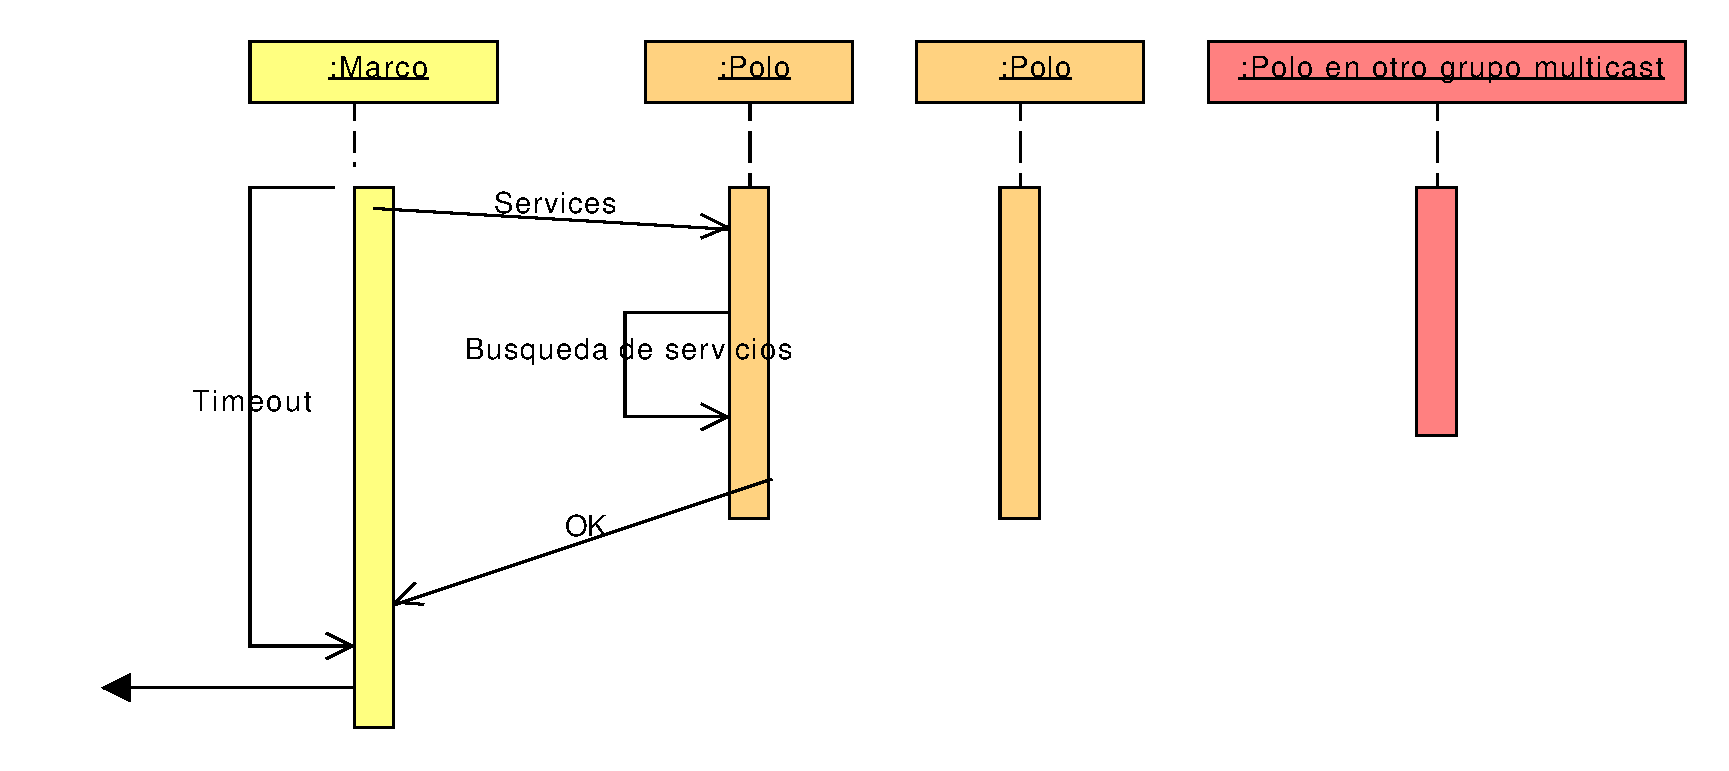
\includegraphics[width=\textwidth]{Diagrams/Sequence/services}
\caption{Diagrama de interacción al enviar el comando \textbf{services}. El nodo al que se le envía el comando consulta la información sobre los servicios que posee y posteriormente envía una respuesta a la instancia de Marco que ha realizado la consulta. Obsérvese toda la información es enviada en modo \textit{unicast}}
\label{fig:secuencia_services}
\end{figure}

\subsection{Arquitectura en detalle}

La funcionalidad del protocolo se segmenta en dos roles claramente definidos e identificados: \textbf{Marco} y \textbf{Polo}. Dicha funcionalidad se implementa en dos ejecutables completamente independientes, que pueden por tanto coexistir o ser ejecutados sin presencia del otro elemento.

Dichos ejecutables son iniciados al arranque el equipo, aprovechando para ello las herramientas que el sistema operativo provee\footnote{Los ejecutables han sido configurados para ser compatibles con el inicializador \textbf{init} y el más reciente \textbf{systemd}.}, y se ejecutan en segundo plano de forma continua (es por ello pueden ser categorizados como procesos \textit{daemon}).

Toda la funcionalidad se ejecuta en un único proceso que se encarga de la creación de los diferentes canales de comunicación (utilizando la API de \textit{sockets} de Berkeley). Dichos canales de comunicación son gestionados por la utilidad \textbf{Twisted}\stepcounter{undefinedreferences}, que simplifica el trabajo con la API, en particular a la hora de crear \textit{sockets} asíncronos.

\subsubsection{Configuración}

Todos los aspectos modificables de cada rol, tales como el grupo \textit{multicast} al que suscribirse o el tiempo de espera predeterminado se definen en un archivo de configuración alojado en el directorio \texttt{/etc/marcopolo} (siguiendo la estructura definida en el \textit{Filesystem Hierarchy Standard} \cite{fhs}).

\begin{figure}[H]
\centering
\VerbatimInput{/home/martin/TFG/Documentación/memoria-tfg/memoria/Code/confdir.txt} %TODO
\caption{Árbol de directorios dentro del directorio de configuración}
\label{fig:arbol_marcopoloconf}
\end{figure}

Los archivos de configuración de cada uno de los \textit{daemons} sigue la típica estructura clave-valor presente en archivos de configuración de servicios del sistema. Por el contrario, la información de todos los servicios a ofrecer sigue la sintaxis de un fichero \textbf{JSON}\footnote{La razón de esta decisión de diseño es la facilidad de interpretación de dicho formato y la legibilidad que ofrecen.}. Todos estos ficheros son leídos al arrancar el ejecutable, y su modificación no tendrá efectos hasta la próxima vez que se inicie el servicio (salvo excepciones que veremos a continuación).

\javascriptcode{statusmonitor}{Un archivo que describe el servicio status monitor}{1}{4}

\subsubsection{Archivos auxiliares}

\paragraph{Log}
Toda la información sobre la ejecución de los \textit{daemons} se refleja en los archivos de \textit{log} presentes en el directorio \texttt{/var/log/marcopolo}. El nivel de log se configura en el parámetro \texttt{LOGLEVEL} de cada uno de los \textit{daemons} y puede tomar uno de los siguientes valores:

\begin{itemize}
\item \textbf{Error} Errores internos durante la ejecución.
\item \textbf{Warn} Advertencias sobre posibles situaciones atípicas.
\item \textbf{Info} Información de interés sobre el funcionamiento del sistema.
\item \textbf{Debug} Información de depuración.
\end{itemize}

%\logcode{/home/martin/TFG/Documentación/memoria-tfg/memoria/Code/marcod}{Caption}{1}{3} %TODO

\paragraph{Registro de ejecución}

En ocasiones es necesario conocer el identificador del proceso \textbf{PID} del \textit{daemon}. Para ello se almacena en el directorio \texttt{/var/run/marcopolo/(marco.pid|polo.pid)} dicho identificador, que puede ser aprovechado por el gestor de arranque del proceso.

\subsection{Integración de los \textit{daemons} en el sistema operativo}

Los \textit{daemons} se integran en el arranque del sistema a través de los ficheros de configuración de \texttt{init}\citationneeded{} o \texttt{systemd} dependiendo del gestor disponible en el sistema operativo sobre el que se ejecuten los procesos.

Por defecto los \textit{daemons} se ejecutan durante todo el ciclo de vida del computador, pero pueden ser reiniciados o detenidos arbitrariamente por voluntad del administrador:

\begin{lstlisting}
systemctl start (marco|polo)
systemctl stop (marco|polo)
systemctl restart (marco|polo)
systemctl reload polo #Orden exclusiva de Polo
\end{lstlisting}

El comando \texttt{reload} permite actualizar la lista de servicios que \textbf{Polo} ofrece sin tener que detener todo el proceso para ello. Dicho comportamiento se consigue de forma similar al comando \texttt{reload} de Apache, enviando la señal \texttt{SIGUSR1} al proceso. 

\subsection{Conexiones con MarcoPolo (\textit{Bindings})}

La funcionalidad de \textbf{MarcoPolo} no se limita al descubrimiento de los servicios del sistema, por lo que es necesario proveer a los usuarios del clúster de herramientas que permitan integrar sus aplicaciones distribuidas con estos servicios. Dichas herramientas, conocidas generalmente como \textit{bindings}, permiten exponer públicamente la funcionalidad de \textbf{MarcoPolo} para que pueda ser aprovechada por otros usuarios.

Se han creado \textit{bindings} para los lenguajes de programación \textbf{Python} y \textbf{Java} y se plantea crear uno para el lenguaje \textbf{C}. Todos ellos son consistentes entre sí, y utilizan la misma sintaxis para realizar el mismo tipo de operación a la vez que aprovechan las características propias de cada lenguaje. Dicha filosofía está inspirada en el funcionamiento de las primitivas de la API de resolución de nombres en red (\texttt{netdb.h})\cite{netdb}, por lo que los \texttt{bindings} se comunican con la instancia local de Marco o Polo a través de \textit{sockets} vinculados a la dirección IP local (127.0.1.1).

Todos los \textit{bindings} deben implementar el mismo conjunto de primitivas, a saber:

\paragraph{Primitivas en el \textit{binding} de Marco}
\begin{itemize}
\item \texttt{request\_for(service, timeout=None)}
Retorna una lista de nodos que ofrecen el servicio indicado en \texttt{service}. Esta función bloquea la ejecución del proceso hasta que el tiempo de espera de nuevas respuestas se cumple (si bien esto no constituye un problema para la mayoría de aplicaciones, es importante que sea conocido por el programador). Si se especifica un \texttt{timeout}, este se utiliza en lugar del determinado por defecto en los parámetros de configuración de \textbf{MarcoPolo}. Se lanza una excepción o un código de error en caso de que la comunicación con la instancia de \textbf{Marco} sea infructuosa (generalmente este tipo de problemas se originan debido a un fallo en el arranque del servicio). Toda la información es transferida en cadenas JSON codificadas en UTF-8.


\item \texttt{getOneNode(criteria=None, timeout=None)}

Retorna un nodo elegido aleatoriamente entre las respuestas (en concreto, el nodo cuya respuesta llegue primero). Si se especifica un criterio en la variable \texttt{criteria} se elegirá el nodo que mejor satisfaga dicho criterio. %TODO in sphinx and MarcoPolo

\item \texttt{getAllNodes(timeout=None)}
Retorna todos los nodos disponibles en la \textit{malla} sin considerar los servicios ofertados. Se lanza una excepción o un código de error en caso de que la comunicación con la instancia de \textbf{Marco} sea infructuosa.

\item \texttt{getNodeInfo(ip)} %TODO Timeout
Obtiene la información de un nodo identificado por su \texttt{ip} si este está disponible en la red.

\end{itemize}

\paragraph{Primitivas en el \textit{binding} de Polo}

\begin{itemize}
\item \texttt{register\_service(service, params=None)}

Añade un nuevo servicio al conjunto de servicios ofertados. El servicio únicamente será ofertado durante el ciclo de vida de la instancia local de Polo. Si esta es detenida o reiniciada se procederá a la eliminación del registro. Para registrar un servicio de forma permanente es necesario definirlo en el directorio \texttt{/etc/marcopolo} %TODO add section reference.

\item \texttt{remove\_service(service)}
Elimina un servicio de la lista de ofertados. Para poder realizar este proceso es necesario ser el ``propietario'' del servicio. Esto es, el único proceso que puede eliminar un servicio es aquel que lo creó o en su defecto la instancia de \textbf{Polo}. En caso de que esta restricción sea quebrantada, una excepción o código de error será retornado.

\item \texttt{have\_service(service)}
Indica si el servicio está ofertado o no.

\end{itemize}

Como se puede observar, la mayoría de primitivas tienen como objetivo el descubrimiento y publicación de servicios. Sin embargo, varias de ellas permiten realizar consultas sobre la información del propio nodo y se plantea la creación de más primitivas que sigan dicha filosofía.

\section{Aplicaciones construidas sobre MarcoPolo}
 
\subsection{Utilidades}

A fin de simplificar al máximo el funcionamiento de los \textit{daemons} varias utilidades que podrían tener cabida dentro del propio protocolo han sido creadas como utilidades independientes que aprovechan la funcionalidad de \textbf{MarcoPolo} para realizar su cometido, pero cuya interdependencia se limita a dichos canales de comunicación.

\subsubsection{\texttt{marcodiscover}}

Esta utilidad consiste en un comando que permite ejecutar consultas al sistema a través de un intérprete de órdenes. El comando posibilita realizar la mayoría de consultas de interés y cuenta con varias opciones para dar diferentes formatos a la salida por pantalla, algo que, como veremos posteriormente, es de gran utilidad para la ejecución de un conjunto particular de programas.

Las opciones del comando son las siguientes:

\begin{figure}[H]
\centering
\begin{lstlisting}
usage: marcodiscover.py [-h] [-d [ADDRESS]] [-s [SERVICE]] [-S [SERVICES]]
                        [-n [NODE]] [--sh [SHELL]]

Discovery of MarcoPolo nodes in the subnet

optional arguments:
  -h, --help            show this help message and exit
  -d [ADDRESS], --discover [ADDRESS]
                        Multicast group where to discover
  -s [SERVICE], --service [SERVICE]
                        Name of the service to look for
  -S [SERVICES], --services [SERVICES]
                        Discover all services in a node
  -n [NODE], --node [NODE]
                        Perform the discovery on only one node, identified by
                        its ip/dns name
  --sh [SHELL], --shell [SHELL]
                        Print output so it can be used as an interable list in
                        a shell

\end{lstlisting}
\caption{Diferentes opciones de configuración de \texttt{marcodiscover}}
\label{fig:marcodiscover_help}
\end{figure}

\subsection{Aplicaciones del sistema}

A fin de aprovechar la funcionalidad de \textbf{MarcoPolo} dentro del sistema, se crean las siguientes utilidades

\subsubsection{Status Monitor}

El monitor de estado consiste en una aplicación con interfaz web que permite observar las estadísticas de uso del \textit{hardware} y de diversos procesos. Utiliza para la detección de los diferentes nodos el \textit{binding} de \textbf{Marco} en Python que realiza una consulta para descubrir que nodos están dispuestos a ofrecer el servicio \texttt{statusmonitor}. La respuesta de dicho comando es enviada al cliente, que establece conexiones directas a cada uno de los nodos a través de \textit{Websockets}\citationneeded. Esto es posible debido a que según la especificación del estándard de websockets, la \textit{Same-Origin Policy}\cite{rfc6455} no es utilizada de la misma forma que en peticiones HTTP,\cite{rfc6454}.

\begin{figure}[H]
\centering
\includegraphics[width=\textwidth]{Diagrams/Sequence/statusmonitor}
\caption{Interacción completa del usuario con \textbf{statusmonitor}. Los mensajes a grupos \textit{multicast} se indican con ``*''}. El usuario se conecta a la página web, que en respuesta envía un código \textit{JavaScript} (además del código HTML y CSS) que solicita la lista de nodos disponibles. Una vez recibida la petición de los nodos disponibles, el servidor solicita dicha información a través de su instancia local de \textbf{Marco} (utilizando para ello un \textit{binding}. Cuando la instancia de \textbf{Marco} termina de recoger las respuestas, retorna la información al servidor, que a su vez retorna dicha información al cliente. Al recibir dicha información, el nodo crea una conexión \textit{Websocket} con el servicio statusmonitor que se encarga de enviar por dicha conexión la información local a intervalos de tiempo definidos.)
\label{fig:secuencia_statusmonitor}
\end{figure}

\begin{figure}[H]
\centering
\includegraphics[width=\textwidth]{Chapter3/Figures/statusmonitor}
\caption{Vista de la interfaz web una vez obtenidos los nodos y establecida la conexión a los mismos. Se observa el porcentaje de memoria y principal y de intercambio utilizadas, la temperatura del procesador, los procesos con más consumo de CPU} %TODO: y el porcentaje de CPU utilizado en cada núcleo.
\label{fig:vista_statusmonitor}
\end{figure}

Para conocer la información sobre el sistema el proceso servidor utiliza varios comandos y ficheros auxiliares, destacando:

\begin{itemize}
\item \texttt{top} Para conocer la información sobre los procesos más activos
\item El directorio \texttt{/proc} para conocer estadísticas del sistema como la memoria total, libre y en caché
\item El directorio \texttt{/sys} para conocer características del hardware como la temperatura
\item Comandos como \texttt{uptime} o \texttt{hostname} para conocer diversos parámetros del sistema.
\item Herramientas como \texttt{awk}, \texttt{grep} o \texttt{cut} para obtener las cadenas de interés dentro del comando de respuesta.
\end{itemize}

Dichos comandos son ejecutados periódicamente mediante el gestor de eventos \texttt{ioloop} de \textbf{Tornado}.

La implementación del servicio está realizada íntegramente en Tornado\footnote{Más información sobre el proyecto puede encontrarse en \href{http://www.tornadoweb.org/en/stable/}{tornadoweb.org/en/stable}}, un servidor web ligero asíncrono implementado íntegramente en Python y mantenido por Facebook.

\subsubsection{Deployer}

El \textbf{Deployer} es una herramienta concebida a partir de la necesidad observada entre los estudiantes de las asignaturas Sistemas Distribuidos y Arquitectura de Computadores (como se refleja en las diferentes evaluaciones\citationneeded %TODO
realizadas), de replicar de una forma sencilla un ejecutable entre los diferentes nodos que conformarán el sistema distribuido.

Actualmente la infraestructura cuenta con un servidor NFS que posibilita la disponibilidad de la información en varios nodos de forma sencilla, mediante la copia a uno de los directorios alojados en el servidor. Sin embargo, este enfoque presenta varios inconvenientes: en el aspecto técnico supone una gran cantidad de ancho de banda consumido de forma continua (debido a que todos los estudiantes utilizan la misma infraestructura y realizan un gran número de operaciones de lectura y escritura a estos directorios, ralentizando el funcionamiento general del sistema enormemente) y en el aspecto didáctico, fomenta un mal hábito, pues los estudiantes no conocen otra forma de realizar despliegues más allá de la copia utilizando una interfaz gráfica y accediendo físicamente al nodo (si bien esta situación se mitiga en la asignatura Sistemas Distribuidos, donde deben automatizar los despliegues). Además, es necesario disponer de acceso físico a cada uno de los nodos, o en su defecto, conocer sus direcciones de red para realizar un acceso remoto.

Con el objetivo de proporcionar una alternativa adecuada a las necesidades y problemas descritos, surge esta herramienta, que aprovecha la funcionalidad de \textbf{MarcoPolo} para realizar su cometido.

La herramienta permite realizar las siguientes tareas de forma sencilla:

\begin{itemize}
\item Conocer todos los nodos disponibles sobre los que se podrá realizar el despliegue y seleccionar sobre cuáles de ellos trabajar.
%\item Conocer la situación de cada nodo en tiempo real, aprovechando la herramienta \textbf{statusmonitor}, cuya funcionalidad se integra en este sistema.
\item Permitir la copia a dichos nodos.
\item Posibilitar la ejecución de comandos de forma remota una vez que el despliegue ha sido realizado.
\item Facilitar la integración con contenedores de servicios, tales como \textbf{Apache Tomcat}.
\end{itemize}

La aplicación es accesible a través de un panel web %TODO: o del comando marcodeploy
. La interfaz web permite además conocer el estado de cada nodo en tiempo real, funcionalidad que a través de la línea de órdenes está disponible a través de los comandos %TODO: marcostatus

\begin{figure}[H]
\centering
\includegraphics[width=\textwidth]{Chapter3/Figures/deployer}
\caption{Interfaz web del deployer. A la izquierda figuran los controles y a la derecha la lista de nodos sobre los que se puede realizar el despliegue}
\label{fig:vista_deployer}
\end{figure}

Al igual que en el caso de la aplicación \textbf{statusmonitor} el \textbf{deployer} está creado utilizando el servidor web \textbf{Tornado} y todo el contenido enviado al usuario se reduce a archivos HTML, CSS y JavaScript. La comunicación entre el cliente y el servidor se realiza a través de peticiones \textit{AJAX} y \textit{Websockets}. Todo el control de la interfaz se delega a hojas de estilo CSS y JavaScript utilizando la biblioteca jQuery\footnote{\href{https://jquery.com/}{jquery.com/}}.

% \begin{figure}[H]
% \centering
% %\includegraphics[width=\textwidth]{Chapter3/Sequence}
% %\caption{Diagrama de secuencia de la interacción}
% %\label{fig:sequence_deployer}
% \end{figure}

\subsection{Pruebas de concepto}

%\includegraphics{Chapter3/ScreenShot.png}http://www.bootc.net/archives/2012/05/26/how-to-build-a-cross-compiler-for-your-raspberry-pi/ % Herramientas

\lhead{Análisis}
\chapter{Análisis}

Recoger todos los aspectos de análisis de un sistema como el creado en un único capítulo es contraproducente para la adecuada comprensión de los diferentes procesos llevados a cabo. Es por ello que en el presente capítulo se detallarán los diferentes aspectos de análisis llevados a cabo para el sistema como unidad, que ayudarán a la identificación de las necesidades a satisfacer por el mismo. Dichos aspectos serán de utilidad durante el desarrollo de las restantes etapas de análisis centradas en cada uno de los diferentes componentes del sistema.

\section{} % Arquitectura

\lhead{\emph{Arquitectura}}
\chapter{Arquitectura}

Sumada a las herramientas creadas en el sistema, es necesario llevar a cabo una serie de operaciones que posibiliten el acceso a servicios más básicos tales como la autenticación de los usuarios del sistema, %TODO etc

Con el objetivo de mejorar la situación actual en la infraestructura a analizar, se tratan los siguientes problemas.

\section{Instalación del sistema}

El sistema a crear requiere de la instalación de diferentes componentes, en particular el sistema operativo, antes de poder ser utilizado. Dicha instalación, si es realizada en cada nodo secuencialmente, implica una gran carga de trabajo y aumenta la propensión a errores durante dicho proceso (en particular si en el mismo existe una gran carga de trabajo que debe ser supervisado por un administrador humano). Una solución a este problema es la autoinstalación del sistema operativo partiendo de una imagen definida y probada por el administrador, que se cargará e instalará en cada nodo sin supervisión.

Una de las herramientas ya existentes para solucionar este problema es el \textbf{PXE} (\textit{Preboox eXecution Environment})\cite{pxeintel}, un estándar \textit{de facto}\cite{avramov:architecture} para la carga de un sistema operativo desde un servidor. El estándar se apoya en protocolos presentes en la práctica totalidad de sistemas, tales como \textbf{DHCP}, \textbf{TFTP} y \textbf{TCP/IP}. El descubrimiento de servicios se realiza mediante una extensión en el mensaje \textbf{DHCPDISCOVER} que envía el servicio \textbf{DHCP} en su secuencia de arranque\cite{rfc4578}. El servidor \textbf{DHCP}, si implementa esta extensión del protocolo, enviará la información sobre la localización de cada uno de los servidores de arranque al cliente, que procederá a la descarga utilizando el protocolo \textbf{TFTP} y posterior instalación\cite{pxeoverview}.

Sin embargo, el uso de este protocolo requiere un controlador de interfaz de red (\textbf{NIC}) en el cliente que soporte el protocolo \textbf{PXE}. Generalmente dicho controlador se incluye como extensión de la \textbf{BIOS} o en equipos más modernos como código \textbf{UEFI}. La \textbf{Raspberry Pi} carece de este tipo de \textit{software}, pues delega todo el arranque del sistema a los datos presentes en la tarjeta SD, y por tanto no es posible realizar ningún tipo de arranque en red sin la previa instalación de un conjunto de aplicaciones que realicen la descarga del sistema operativo. Es por ello que el uso de \textbf{PXE} como herramienta de arranque debe ser desestimado.

\subsection{marco-netinst}

Debido a la falta de soporte para \textbf{PXE} u otra alternativa similar, es necesario crear una herramienta que se encargue de la detección de un servidor que aloje la imagen del sistema operativo, la descarga del mismo y su instalación. Con este objetivo se crea la herramienta \textbf{marco-netinst}.

\textbf{marco-netinst} es una ramificación del proyecto \textbf{rasbpian-ua-netinst}\cite{raspbian-ua-netinst}. Esta utilidad permite instalar un conjunto mínimo de utilidades que posibilitan la descarga de un sistema operativo desde los repositorios de \textbf{Debian} y su instalación. La ramificación incluye las siguientes modificaciones:

\begin{itemize}
	\item Instalación de \textbf{ArchLinux ARM} en lugar de \textbf{Raspbian}.
	\item Instalación del sistema operativo completo a partir de un archivo \textbf{.tar.gz} en lugar de la descarga de paquetes\footnote{\textbf{raspbian-ua-netinst} utiliza el paquete cdebootstrap-static para la descarga e instalación de todos los archivos. Existe una herramienta para ArchLinux similar, denominada \textbf{Archbootstrap}\\
	\href{https://wiki.archlinux.org/index.php/Archbootstrap}{https://wiki.archlinux.org/index.php/Archbootstrap}\\
	\href{https://packages.debian.org/sid/cdebootstrap-static}{https://packages.debian.org/sid/cdebootstrap-static}}.
	\item Nuevo \textit{script} de carga del \textit{software} en la tarjeta SD (en el paquete original se delega a utilidades de terceros).
	%TODO\item Posibilidad de aplicar diferentes esquemas de particionado
	\item Detección del servidor sin configuración previa utilizando \textbf{MarcoPolo}.
	%TODO\item Interfaz administrativa de los sistemas operativos ofrecidos
\end{itemize}

La especificación en detalle del funcionamiento de la herramienta se detalla en el anexo%TODOf

\section{Autenticación de los usuarios}

Los usuarios del sistema deben ser capaces de acceder al sistema mediante un sistema de credenciales que posibilite el uso de cualquier nodo del sistema con el mismo conjunto de claves. Dicho enfoque es el propio de la infraestructura actual del sistema, que en concreto sigue un enfoque centralizado.

Un primer intento de posibilitar la ``universalización'' del acceso ha sido la creación de los mismos usuarios en cada uno de los nodos, utilizando el mismo par usuario-contraseña en cada uno de ellos. Sin embargo, este enfoque impide una escalabilidad sencilla y requiere un mantenimiento continuo (suponiendo que se añaden usuarios periódicamente). Por ello únicamente las pruebas iniciales de las plataformas que requieren acceso a la funcionalidad de autenticación han sido realizadas siguiendo este enfoque, pero siempre desacoplando al máximo el sistema de acceso del resto de la lógica del programa, con el objetivo de facilitar su reemplazo.

Habiendo descartado dicha estrategia, queda como alternativa más adecuada a las necesidades del sistema el uso de la infraestructura presente en el centro académico.

La infraestructura del centro comprende varios servicios que interactúan entre sí, siendo el pilar clave el servidor LDAP (\textit{Lightweight Directory Access Protocol})\citationneeded. Dicho servidor almacena la información de todos los usuarios de la infraestructura y da acceso a cualquier equipo de varias de las aulas de la Facultad.
\begin{figure}[H]
	\centering
	\includegraphics[width=0.7\textwidth]{Chapter5/Figures/LDAP.pdf}
	\caption{Esquema de los diferentes componentes del sistema de autenticación y gestión de archivos, así como de una serie de componentes adicionales. Obsérvese la interacción entre los componentes situados en el rectángulo interior}
	\label{fig:arquitectura_ldap}
\end{figure}

\subsection{Características en detalle}

Debido a la heterogeneidad de los diferentes equipos presentes en la infraestructura, el sistema debe posibilitar el acceso a todos los equipos utilizando el mismo conjunto de credenciales. Esto implica que el sistema debe ser compatible con al menos los sistemas operativos GNU/Linux, Microsoft Windows y Solaris. Por ello se interconecta el servidor LDAP con Samba, así como el PAM (\textit{Pluggable Authentication Module}) tanto en el cliente como el servidor.

Sin embargo el sistema permite también que los usuarios puedan almacenar información en un espacio centralizado al que es posible acceder desde cualquier equipo, facilitando la copia de ficheros entre nodos, uniformidad de los diferentes equipos. Esto se consigue utilizando un servidor NFS (\textit{Network File Storage}).

\subsection{Utilización en el sistema}

En el sistema se aprovechará principalmente la funcionalidad de autenticación provista por el servidor LDAP, debido a que uno de los objetivos principales del sistema es evitar ``cuellos de botella'' debido al uso de un servidor de almacenamiento central. Herramientas como el \textbf{deployer} facilitarán la replicación de servicios en su lugar. En cualquier caso, se plantea permitir el acceso al NFS desde el sistema como complemento, pero no como espacio principal de almacenamiento.

El sistema aprovecha el módulo PAM para realizar el proceso de autenticación.

\section{Compilación}

Si bien el sistema Raspberry Pi es capaz de compilar el \textit{software} que después utilizará, en ocasiones es beneficioso delegar dicha tarea a otro componente que realice el proceso por el nodo en cuestión y posteriormente añadir los archivos ejecutables al sistema. Este enfoque reduce el tiempo de trabajo de forma significativa, como observaremos posteriormente.%proporcione los resultados al solicitante.

\subsection{Creación de un compilador cruzado}

Un compilador cruzado (\textit{cross-compiler})es una herramienta capaz de generar código para una architectura utilizando un equipo con otra arquitectura diferente.%TODO: http://en.wikipedia.org/wiki/Cross_compiler
El uso de compiladores cruzados 

\subsection{Análisis del rendimiento}

Para determinar el rendimiento del compilador se ha utilizado el mismo en la compilación de diferentes herramientas a utilizar en el sistema:

\subsubsection{OpenMPI}

\textbf{Tiempo de compilación en Rasbperry Pi}: 4447 seconds (1 h y 14 minutos)

\textbf{Tiempo de compilación con el compilador cruzado sin paralelización}: 2710 seconds (45 minutos)

\textbf{Tiempo de compilación con 4 trabajos paralelos (make -j4)}: 1267 seconds (21 minutos) % Herramientas de terceros

\lhead{\emph{Arquitectura software}}
\chapter{Arquitectura software}

Con el objetivo de facilitar la comprensión del sistema como un todo esta memoria se estructura partiendo de los cimientos del sistema, ascendiendo hasta las aplicaciones de más alto nivel manipuladas por los usuarios, describiendo de forma exhaustiva todos los aspectos de relevancia y esfuerzos llevados a cabo para diseñar y desarrollar cada uno de los componentes del sistema.

\section{Sistema operativo}

Una pieza fundamental del \textit{software} del sistema es la capa más básica del mismo, el sistema operativo. Es por ello clave elegir un sistema adecuado para los objetivos que se desean alcanzar.

Como se describió en \ref{problema:sistemaoperativo}, se utilizará el sistema operativo Arch Linux en su variante para procesadores ARM por su diseño altamente modular, eficiencia y capacidad de adaptabilidad. Sobre dicho sistema operativo se desarrollarán el resto de componentes, sin que ello implique un diseño adaptado a este sistema operativo.

\subsection{Características técnicas de Arch Linux}
\label{archlinux:description}

\textbf{Arch Linux} es una distribución del sistema operativo GNU/Linux creada y mantenida por una comunidad de usuarios. Desarrollada de forma independiente, es lo suficientemente versátil como para satisfacer cualquier propósito. Su desarrollo se centra en la simplicidad, elegancia y minimalismo, asumiendo que el usuario añadirá los componentes que restan para conseguir el entorno que desee. Dicho minimalismo se traduce en una arquitectura basada en paquetes que conforman en su conjunto un sistema fácil de comprender por el usuario, y que cuentan con una gran cantidad de documentación fácilmente accesible. La consecuencia directa de este minimalismo es el rendimiento del sistema. Una instalación de Arch Linux se limita al conjunto de paquetes mínimo para contar con un sistema completamente funcional, delegando al usuario la adición de nuevos paquetes. Este enfoque permite optimizar de forma sencilla el rendimiento del sistema, al no contar con paquetes innecesarios.

Arch Linux está basado en un modelo de liberación continua (\textit{rolling release}) lo cual significa que el sistema está en constante desarrollo (en contraste con un sistema de versiones). El \textit{software} se actualiza de forma continua, siendo únicamente necesario realizar una actualización de los paquetes que conforman el sistema para contar con la última versión. Este modelo de desarrollo permite contar con las últimas versiones del software incluido de forma casi inmediata a su liberación. Generalmente los paquetes que se incluyen sin modificaciones por parte del proyecto (esta práctica se denomina \textit{upstream}, pues la fuente del software es el propio autor del mismo), tal y como el fueron creados para su uso.

La gestión de paquetes se realiza utilizando la herramienta \textbf{pacman}\cite{pacman}, creada por y para el proyecto. El repositorio oficial ofrece una gran cantidad de paquetes, si bien su tamaño es significativamente inferior al \textit{Arch User Repository} (AUR), que contiene paquetes creados y mantenidos por usuarios.

Arch Linux utiliza el sistema de arranque \textbf{systemd}\cite{systemd}, un conjunto de módulos que proporcionan una gestión de dependencias entre servicios del sistema más eficiente y sencilla que el cargador clásico de las distribuiciones GNU, \textbf{init}\cite{init}, inspirado en el utilizado por UNIX System V.

Otro de los aspectos de relevancia del sistema es la comunidad creada alrededor del mismo, que fomenta la implicación de cualquier usuario en cualquiera de los aspectos de relevancia en el desarollo del sistema. La documentación del sistema es extensa y cuenta con recursos tanto para las características propias del sistema como para herramientas de terceros utilizadas en el mismo. %Además, la comunidad de Arch Linux es famosa por la gran y exhaustiva cantidad de documentación que mantiene, así como las diferentes opciones de soporte a cualquier nivel que ofrece a través de diferentes canales.

Dichos aspectos del proyecto y una serie de consideraciones adicionales se recogen en los preceptos definidos en el documento \textit{The Arch Way}\cite{thearchway}, inspirado en el principio de desarrollo \textbf{KISS} (\textit{Keep It Simple, Stupid}), muy popular en el entorno de los sistemas operativos UNIX.%\citationneeded{http://people.apache.org/~fhanik/kiss.html}. 

Arch Linux ARM\footnote{\href{http://archlinuxarm.org/}{http://archlinuxarm.org/}} es un proyecto derivado de Arch Linux que tiene como objetivo portar el sistema operativo a dispositivos basados en la arquitectura ARM (pues el proyecto raíz está enfocado únicamente en las arquitecturas i686 y x68\_64), generalmente sistemas embebidos, habiendo conseguido la compatibilidad con las versiones v5te, v6h y v7h de la arquitectura. El proyecto mantiene la misma filosofía de diseño que su progenitor, siendo el buen rendimiento del sistema operativo uno de los aspectos que propician el uso de esta distribución en sistemas con un capacidad de cómputo reducida. Es una de las principales opciones a la hora de realizar proyectos con este tipo de computadores\cite{distrowatch:arm}.%TODO: Revisar



%Además, Arch Linux apuesta por un modelo de desarrollo de liberación continua (\textit{rolling releases}). El sistema operativo no se distribuye en versiones, sino en imágenes con las últimas versiones de los paquetes disponibles, lo cual posibilita contar con las últimas versiones de las herramientas presentes en el sistema operativo poco tiempo (o de forma inmediata) a su liberación. El modelo de desarrollo sigue este principio de forma tan estricta, que basta una actualización de todos los paquetes del sistema mediante el gestor propio de la distribución (\textbf{pacman}) para actualizar el sistema operativo (en contraste con operaciones específicas para este cometido, como ocurre con otros sistemas operativos).

%El sistema operativo delega la responsabilidad del mantenimiento de todos los componentes al usuario en un grado mayor que el que pueden ofrecer otras distribuciones. Esto permite a los usuarios contar con completa libertad para modificar componentes del sistema en función de sus intereses a cualquier nivel\citationneeded{https://wiki.archlinux.org/index.php/The\_Arch\_Way}.


El proceso de elección del sistema operativo puede observarse en \ref{os:evaluation}.


\subsection{Sistema operativo en el servidor}

En el caso del servidor que provee diferentes servicios de apoyo a los nodos principales (ver \ref{sistema:arquitectura}) se utiliza el sistema operativo Debian GNU/Linux. Este sistema operativo tiene como objetivo la estabilidad del sistema en detrimento de las últimas características del \textit{software} que lo conforma.

\section{Servicios integrados en el sistema operativo}

Diversos componentes del sistema operativo son utilizados para llevar a cabo operaciones de gestión o como herramienta para la creación de aplicaciones en niveles superiores. Gracias a la integración de estos componentes en niveles inferiores, es posible ofrecer dichos servicios a cualquier aplicación de usuario. 


\subsection{Gestión de servicios}

\textbf{systemd} es utilizado como gestor de los diferentes servicios del sistema, así como aquellos creados en el proceso de desarrollo del mismo. Se aprovecha su capacidad para gestionar dependencias entre los diferentes componentes (orden de arranque, qué servicios deben arrancarse para que otros puedan funcionar\dots) para establecer el orden de inicio al arrancar el sistema o iniciar automáticamente servicios sobre los que dependan otros.

\textbf{systemd} define cada uno de los diferentes servicios (``unidades'') en un fichero independiente.

\section{Descubrimiento de servicios: el protocolo MarcoPolo}

Uno de los problemas típicos a la hora de crear un sistema distribuido es la localización de cada uno de los nodos que lo conforman. Al no existir un coordinador, es difícil establecer un mecanismo de interconexión entre los diferentes nodos que sea escalable e independiente de factores externos (e.g. IP asignada en un momento dado, número de nodos en la red).


Soluciones como el uso de servidores de nombres (\textbf{DNS}) permiten crear estructuras jerárquicas donde cada nodo está identificado por un nombre previamente asignado y conocido. Como primera propuesta de solución se plantea el uso de los nombres de equipo que el servidor \textbf{DHCP} presente en la infraestructura otorga. Con esta solución los nodos serían accesibles mediante un identificador invariable en el tiempo (en contraste con una IP dinámica). Sin embargo, dicha solución presenta un grave problema en materia de escalabilidad: no existe un ``directorio'' que recoja qué nodos están activos en un momento dado ni que refleje adiciones en la lista original de nodos, por lo que para poder realizar cualquier cambio en el conjunto de nodos del sistema será necesario configurar cada equipo manualmente. También existen protocolos inspirados en enfoque como \textbf{mDNS} (\textit{Multicast Domain Name Service}) donde la necesidad de un servidor de nombres desaparece, y los nodos son capaces de realizar el descubrimiento mediante mensajes uno-a-muchos\cite{rfc6762}. Implementaciones de este protocolo, como \textit{Bonjour}, \textit{Avahi} o \textit{AppleTalk} (ya descontinuado) han sido evaluadas a la hora de buscar una solución a este problema. Sin embargo, estas y otras soluciones similares no responden a una de las necesidades básicas del sistema a construir: la condición de que la información que conoce cada nodo sobre el resto en el arranque del sistema es nula. Si bien con \textbf{mDNS} desaparece la necesidad con un servidor de nombres y es posible realizar operaciones de descubrimiento de servicios, este y otros protocolos similares asumen que la información de un nodo presente de una red local es de interés para el resto de miembros de la misma, lo cual dificulta la independencia de un conjunto de equipos frente al resto en el mismo espacio de direcciones.

%Avahi?

\subsection{MarcoPolo, el protocolo de descubrimiento de servicios}
\label{marcopolo}

Una de las características clave del sistema consiste en la escalabilidad del mismo en tiempo de ejecución: no es necesario conocer qué nodos participan en el sistema hasta que no se requiera de los mismos. Además, se pretende optimizar al máximo cada uno de los nodos del sistema por separado, por lo que designar a uno de ellos como ``autoridad'' frente a la que el resto de nodos se registren y esta actúe posteriormente como coordinador y \textit{``resolver''} supone una dedicación de recursos innecesaria y que dificulta la escalabilidad del sistema. Además, la gestión del espacio de direcciones de la red en la que se integra el sistema, que es compartido con una gran cantidad de equipos adicionales, no recaería en dicho coordinador. Esto implica que las direcciones de cada nodo son asignadas por un servidor DHCP sobre el que no se tiene control y cuyas asignaciones son dadas por intervalos de tiempo pequeños\footnote{Durante el desarrollo del sistema se observa que las direcciones son asignadas por periodos de tiempo pequeños y no suelen repetirse a menos que dicha dirección no haya sido asignada anteriormente, fenómeno que suele darse con bastante frecuencia.}. %TODOEsto implica que no es posible contar con un nodo coordinador sin un espacio de nombres anteriormente definido.
Por otro lado, la clave de este sistema no la constituye la disponibilidad de un nodo, sino las aplicaciones distribuidas que pueden utilizarse en el mismo (de ahora en adelante serán denominadas ``servicios''). Un nodo puede contar con un conjunto de servicios diferente al de sus vecinos, y por tanto colaborará en unas tareas y en otras no en virtud de dicha disponibilidad.%TODO Este requisito no es satisfecho por la mayoría de los sistemas anteriormente mencionados.

Motivada por esta serie de características surge la necesidad de crear un protocolo de descubrimiento de nodos y servicios basado principalmente en los servicios que dichos nodos pueden (y desean) ofrecer. Además, siendo uno de los objetivos funcionales del sistema el aprovechamiento del mismo como herramienta didáctica, surge la necesidad de que dos conjuntos de nodos puedan trabajar en la misma red de forma independiente. Como aproximación para satisfacer estas necesidades surge el procolo de descubrimiento de servicios \textbf{MarcoPolo}.

\subsubsection{Introducción}

\textbf{MarcoPolo} es un protocolo de descubrimiento de servicios cuya dinámica y nombre se inspiran en el juego homónimo\footnote{\href{https://en.wikipedia.org/wiki/Marco\_Polo\_\%28game\%29}{https://en.wikipedia.org/wiki/Marco\_Polo\_\%28game\%29}}, en el cual uno de los integrantes debe encontrar al resto privado de visión mediante ecolocalización (gritando la palabra clave ``Marco'', cuya respuesta por parte del resto de jugadores es ``Polo''). El protocolo se compone de dos roles claramente diferenciados (e independientes aún siendo ejecutados en el mismo nodo): \textbf{Marco}, encargado de enviar consultas a la red y \textbf{Polo}, que emite una respuesta a dichos comandos y gestiona la información de cada nodo. %TODO: 

Con el objetivo de posibilitar la coexistencia de varias ``mallas'' de nodos independientes (donde los servicios ofrecidos por un nodo sean conocidos y consecuentemente aprovechables únicamente por el resto) a la vez que las consultas son realizadas a todos los integrantes sin necesidad de conocer su identificador en la red (dirección a nivel de red o enlace, nombre \textbf{DNS}) se utilizan mensajes uno-a-muchos, conocidos con el nombre \textit{multicast}, donde cada una de las ``mallas'' se comunicará con el resto de integrantes de la misma a través de un grupo preestablecido (o consensuado por dichos nodos).

\subsubsection{Funcionamiento}

El protocolo se basa en el envío de mensajes a un grupo multicast acordado previamente (existiendo un grupo designado por defecto). Los nodos suscritos a dicho grupo recibirán dicho mensaje y lo procesarán, emitiendo una respuesta dirigida únicamente al nodo que ha realizado la solicitud en caso de que el mensaje solicite un servicio que el nodo ofrezca. En caso contrario no se emitirá ninguna respuesta. Dicho mensaje incluirá información adicional, como el método de acceso al servicio, estado del nodo, etcétera.

El solicitante esperará durante un tiempo pequeño a que haya respuesta por parte del resto de nodos, recogiendo todos los mensajes recibidos. Una vez que el tiempo de espera haya pasado, se retornarán los resultados al programa o usuario solicitante.

\subsection{Comandos}

Los mensajes utilizados se denominan \textit{comandos} y contienen las consultas sobre un servicio, nodo o información sobre la propia \textit{malla} que se desea conocer, así como la respuesta a dichas consultas. Dichos comandos son enviados como cadenas de texto que almacenan la información en estructuras de datos JSON (\textit{JavaScript Object Notation}) debido a la gran legibilidad de estas por humanos y máquinas, y la popularidad de este formato como mecanismo de transmisión de informaciónla gran cantidad de herramientas disponibles para su creación y procesado.

Los comandos de MarcoPolo constituyen las primitivas del protocolo. Actualmente se cuenta con las siguientes primitivas y las correspondientes respuestas:
\begin{landscape}
\begin{table}[H]
\begin{tabular}{|p{2.35cm}|p{1.2cm}|p{4.5cm}|p{5cm}|p{5cm}|p{3.5cm}|}
\hline
\textbf{Nombre} & \textbf{Emisor} & \textbf{Función} & \textbf{Información} & \textbf{Respuesta esperada} & \textbf{Protocolo}\\ \hline

\textbf{Marco} & Marco & Descubrir todos los nodos presentes en la malla & Únicamente se incluye el nombre del comando & Un comando \textit{Polo} por cada nodo disponible en la red o ninguna si no existe ningún nodo. & UDP \textit{multicast} al puerto 1338.\\ \hline

\textbf{Polo} & Polo & Notificar de la presencia de este nodo al recibir un mensaje \textbf{marco} & Información opcional sobre el nodo (e.g. estado, \textit{hostname}\dots), incluyendo opcionalmente información adicional  & Ninguna &  UDP \textit{unicast} al puerto efímero del nodo solicitante.\\ \hline

\textbf{Request-For} & Marco & Conocer todos los nodos que ofrecen un servicio a través de su identificador único en el sistema & Identificador del servicio a descubrir & Un mensaje \textit{OK} con información opcional sobre el nodo o el servicio & UDP \textit{multicast} al puerto 1338.\\ \hline

\textbf{OK} & Polo & Comando utilizado para emitir una respuesta a una petición. & Respuesta a un comando con la información solicitada & Ninguna & UDP \textit{unicast} al puerto efímero de la pregunta.\\ \hline

\textbf{Services} & Marco & Descubrir todos los servicios ofrecidos por un nodo & No se envía información adicional con el comando & \textbf{OK} con una lista de los identificadores del servicio o ninguna si el nodo no se encuentra activo. & UDP \textit{unicast} al puerto 1338.\\ \hline
\end{tabular}
\caption{Comandos del protocolo MarcoPolo}
\end{table}
\end{landscape}

\subsection{Esquemas de comunicación}

\subsubsection{Comando \textbf{Marco}}

%TODO \begin{figure}[H]
% \centering
% \includegraphics[width=\textwidth]{Diagrams/Sequence/marcocompleto}
% \caption[Interacción al enviar el comando \textbf{Marco}]{Interacción al enviar el comando \textbf{Marco}. Los mensajes a grupos \textit{multicast} se indican con ``*''}
% \label{fig:secuencia_marco}
% \end{figure}

El comando Marco se envía al grupo \textit{multicast} definido en la configuración de la instancia local de \textbf{Marco} o a aquel definido en tiempo de ejecución. Los nodos suscritos a dicho grupo (aquellos que pertenecen a la malla) reciben el mensaje y emiten una respuesta \textbf{Polo}. Debido a la falta de una conexión entre los nodos (todos los mensajes son intercambiados utilizando el protocolo \textbf{UDP}) se fija un tiempo de espera, durante el cual se reciben y acumulan todas las respuestas. Al pasar dicho tiempo, se retornan los resultados y los mensajes recibidos posteriormente son ignorados.

% TODO\begin{figure}[H]
% 	\centering
% 	\includegraphics[width=\textwidth]{Diagrams/Sequence/request_for}
% 	\caption[Interacción al enviar el comando \textbf{Request-For}]{Diagrama de interacción al enviar el comando \textbf{Request-For}. Los nodos comprueban si deben ofrecer el servicio identificado por la clave \textit{s}. En caso de que la búsqueda sea exitosa se retorna un mensaje indicando la disponibilidad de dicho nodo. En caso contrario no habrá respuesta alguna.
% 	Los mensajes enviados a grupos \textit{multicast} se indican con ``*''}
% 	\label{fig:secuencia_request_for}
% \end{figure}

% TODO\begin{figure}[H]
% 	\centering
% 	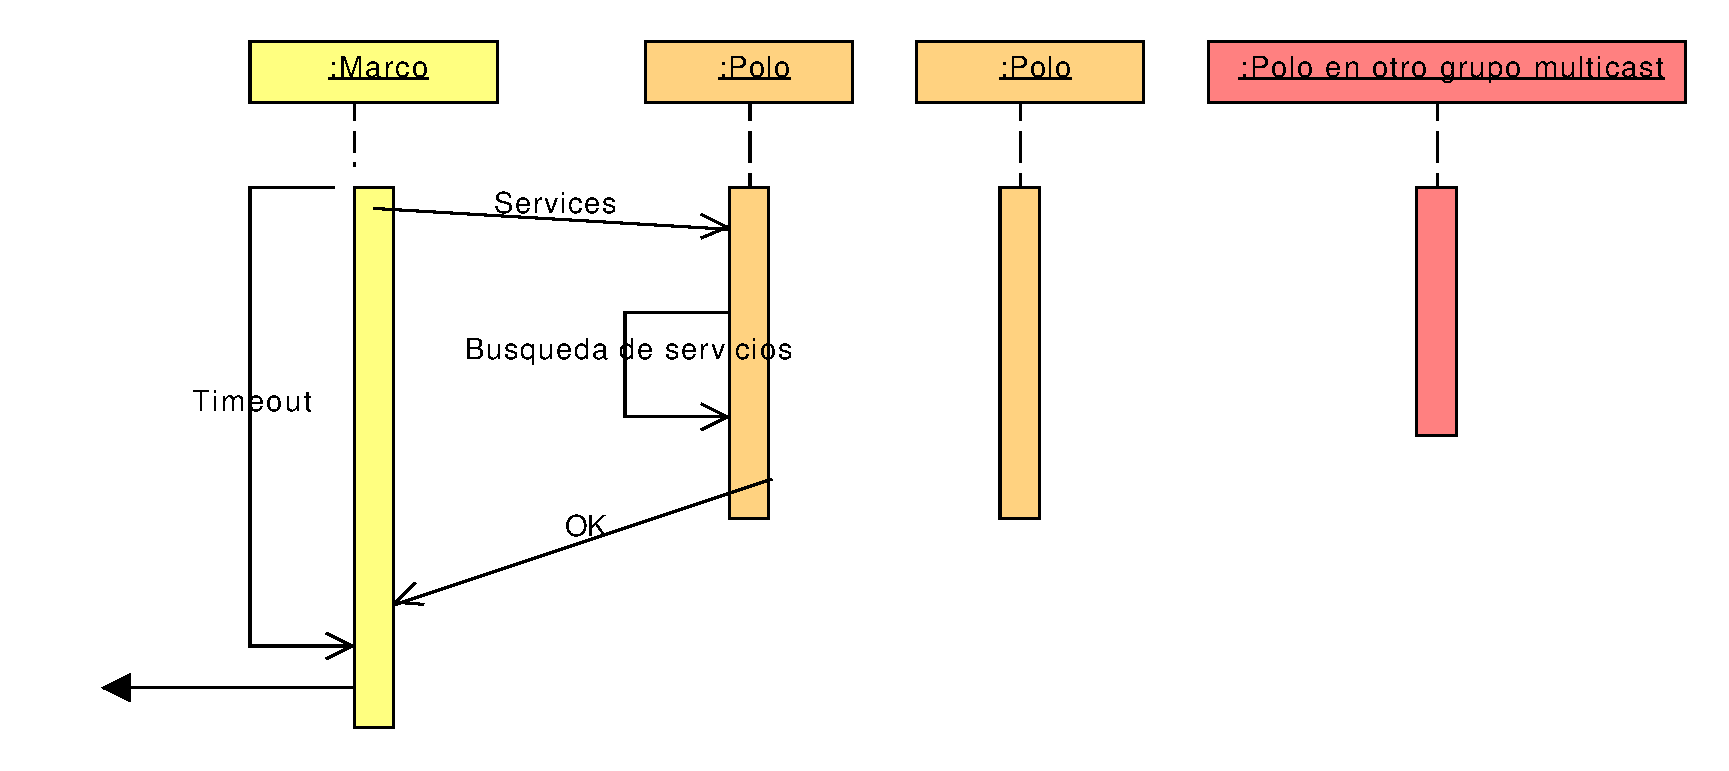
\includegraphics[width=\textwidth]{Diagrams/Sequence/services}
% 	\caption[Diagrama de interacción al enviar el comando \textbf{Services}]{Diagrama de interacción al enviar el comando \textbf{Services}. El nodo al que se le envía el comando consulta la información sobre los servicios que posee y posteriormente envía una respuesta a la instancia de Marco que ha realizado la consulta. Obsérvese toda la información es enviada en modo \textit{unicast}}
% 	\label{fig:secuencia_services}
% \end{figure}

\subsection{Arquitectura en detalle}

La funcionalidad del protocolo se segmenta en dos roles claramente definidos e identificados: \textbf{Marco} y \textbf{Polo}. Dicha funcionalidad se implementa en dos ejecutables completamente independientes, que pueden por tanto coexistir o ser ejecutados sin presencia del otro.

Estos ejecutables están diseñados para ser iniciados al arranque el equipo, aprovechando para ello las herramientas que el este provee\footnote{Los ejecutables han sido configurados para ser compatibles con los gestores de arranque \textbf{init} y el más reciente \textbf{systemd}.}, y se ejecutan en segundo plano de forma continua (es por ello pueden ser categorizados como procesos \textit{daemon}).

Toda la funcionalidad se ejecuta en un único proceso que se encarga de la creación de los diferentes canales de comunicación (utilizando la API de \textit{sockets} de Berkeley). Dichos canales de comunicación son gestionados por la utilidad \textbf{Twisted}\footnote{\href{https://twistedmatrix.com/trac/}{https://twistedmatrix.com/trac/}}, que simplifica el trabajo con la API, en particular a la hora de crear \textit{sockets} asíncronos.

\subsubsection{Configuración}

Todos los aspectos modificables de cada rol, tales como el grupo \textit{multicast} al que suscribirse o el tiempo de espera predeterminado se definen en un archivo de configuración alojado en el directorio \texttt{/etc/marcopolo} (siguiendo la estructura definida en el \textit{Filesystem Hierarchy Standard} \cite{fhs}).

% \begin{figure}[H]
% 	\centering
% 	\VerbatimInput{/home/martin/TFG/Documentación/memoria-tfg/memoria/Code/confdir.txt} %TODO
% 	\caption{Árbol de directorios dentro del directorio de configuración}
% 	\label{fig:arbol_marcopoloconf}
% \end{figure}

Los archivos de configuración de cada uno de los \textit{daemons} sigue la típica estructura clave-valor presente en archivos de configuración de servicios del sistema. Por el contrario, la información de los servicios a ofrecer sigue la sintaxis de un fichero \textbf{JSON}\footnote{La razón de esta decisión de diseño es la facilidad de interpretación de dicho formato y la legibilidad que ofrecen.}. Todos estos ficheros son leídos al arrancar el ejecutable, y su modificación no tendrá efectos hasta la próxima vez que se inicie el servicio.%TODO (salvo excepciones que veremos a continuación).

\javascriptcode{statusmonitor}{Un archivo que describe el servicio status monitor}{1}{7}

\subsubsection{Archivos auxiliares}

\paragraph{Log}
Toda la información sobre la ejecución de los \textit{daemons} se refleja en los archivos de \textit{log} presentes en el directorio \texttt{/var/log/marcopolo}. El nivel de log se configura en el parámetro \texttt{LOGLEVEL} de cada uno de los \textit{daemons} y puede tomar uno de los siguientes valores:

\begin{itemize}
\item \textbf{Error} Errores internos durante la ejecución.
\item \textbf{Warn} Advertencias sobre posibles situaciones atípicas.
\item \textbf{Info} Información de interés sobre el funcionamiento del sistema.
\item \textbf{Debug} Información de depuración.
\end{itemize}

%\logcode{/home/martin/TFG/Documentación/memoria-tfg/memoria/Code/marcod}{Caption}{1}{3} %TODO

\paragraph{Registro de ejecución}

En ocasiones es necesario conocer el identificador del proceso \textbf{PID} del \textit{daemon}. Para ello se almacena en el directorio \texttt{/var/run/(marcod.pid|polod.pid)} dicho identificador, que puede ser aprovechado por el gestor de arranque del proceso.

\subsection{Integración de los \textit{daemons} en el sistema operativo}

Los \textit{daemons} se integran en el arranque del sistema a través de los ficheros de configuración de \texttt{init}\footnote{\href{http://www.tldp.org/HOWTO/HighQuality-Apps-HOWTO/boot.html}{http://www.tldp.org/HOWTO/HighQuality-Apps-HOWTO/boot.html}} o \texttt{systemd} dependiendo del gestor disponible en el sistema operativo sobre el que se ejecuten los procesos. Por defecto los \textit{daemons} se ejecutan durante todo el ciclo de vida del computador, pero pueden ser reiniciados o detenidos arbitrariamente por voluntad del administrador.

% TODO: para el documento en detalle \begin{lstlisting}
% systemctl start (marco|polo)
% systemctl stop (marco|polo)
% systemctl restart (marco|polo)
% systemctl reload polo #Orden exclusiva de Polo
% \end{lstlisting}

% El comando \texttt{reload} permite actualizar la lista de servicios que \textbf{Polo} ofrece sin tener que detener todo el proceso para ello. Dicho comportamiento se consigue de forma similar al comando \texttt{reload} de Apache, enviando la señal \texttt{SIGUSR1} al proceso. 

\subsection{Conexiones con MarcoPolo}

La funcionalidad de \textbf{MarcoPolo} no se limita al descubrimiento de los servicios del sistema, por lo que es necesario ofrecer a los usuarios del clúster herramientas que permitan integrar sus aplicaciones distribuidas con estos servicios. Dichas herramientas, conocidas como \textit{bindings}, permiten exponer públicamente la funcionalidad de \textbf{MarcoPolo} para que pueda ser aprovechada por otros usuarios.

Se han creado \textit{bindings} para los lenguajes de programación \textbf{C}, \textbf{C++}, \textbf{Python} y \textbf{Java}. Todos ellos son consistentes entre sí, manteniendo la misma sintaxis para realizar el mismo tipo de operación a la vez que aprovechan las características propias de cada lenguaje. Dicha filosofía está inspirada en el funcionamiento de las primitivas de la API de resolución de nombres en red (\texttt{netdb.h})\cite{netdb}, por lo que los \texttt{bindings} se comunican con la instancia local de Marco o Polo a través de \textit{sockets} vinculados a la dirección IP local (127.0.1.1).

Todos los \textit{bindings} deben implementar el mismo conjunto de primitivas, definidas en la documentación de refencia de MarcoPolo (ver anexo). La mayoría de primitivas tienen como objetivo el descubrimiento y publicación de servicios. Sin embargo, varias de ellas permiten realizar consultas sobre la información del propio nodo y se plantea la creación de más primitivas que sigan dicha filosofía

%TODO \paragraph{Primitivas en el \textit{binding} de Marco}
% \begin{itemize}
% \item \texttt{request\_for(service, timeout=None)}
% Retorna una lista de nodos que ofrecen el servicio indicado en \texttt{service}. Esta función bloquea la ejecución del proceso hasta que el tiempo de espera de nuevas respuestas se cumple (si bien esto no constituye un problema para la mayoría de aplicaciones, es importante que sea conocido por el programador). Si se especifica un \texttt{timeout}, este se utiliza en lugar del determinado por defecto en los parámetros de configuración de \textbf{MarcoPolo}. Se lanza una excepción o un código de error en caso de que la comunicación con la instancia de \textbf{Marco} sea infructuosa (generalmente este tipo de problemas se originan debido a un fallo en el arranque del servicio). Toda la información es transferida en cadenas JSON codificadas en UTF-8.


% \item \texttt{getOneNode(criteria=None, timeout=None)}

% Retorna un nodo elegido aleatoriamente entre las respuestas (en concreto, el nodo cuya respuesta llegue primero). Si se especifica un criterio en la variable \texttt{criteria} se elegirá el nodo que mejor satisfaga dicho criterio. %TODO in sphinx and MarcoPolo

% \item \texttt{getAllNodes(timeout=None)}
% Retorna todos los nodos disponibles en la \textit{malla} sin considerar los servicios ofertados. Se lanza una excepción o un código de error en caso de que la comunicación con la instancia de \textbf{Marco} sea infructuosa.

% \item \texttt{getNodeInfo(ip)} %TODO Timeout
% Obtiene la información de un nodo identificado por su \texttt{ip} si este está disponible en la red.

% \end{itemize}

% \paragraph{Primitivas en el \textit{binding} de Polo}

% \begin{itemize}
% \item \texttt{register\_service(service, params=None)}

% Añade un nuevo servicio al conjunto de servicios ofertados. El servicio únicamente será ofertado durante el ciclo de vida de la instancia local de Polo. Si esta es detenida o reiniciada se procederá a la eliminación del registro. Para registrar un servicio de forma permanente es necesario definirlo en el directorio \texttt{/etc/marcopolo} %TODO add section reference.

% \item \texttt{remove\_service(service)}
% Elimina un servicio de la lista de ofertados. Para poder realizar este proceso es necesario ser el ``propietario'' del servicio. Esto es, el único proceso que puede eliminar un servicio es aquel que lo creó o en su defecto la instancia de \textbf{Polo}. En caso de que esta restricción sea quebrantada, una excepción o código de error será retornado.

% \item \texttt{have\_service(service)}
% Indica si el servicio está ofertado o no.

% \end{itemize}

% Como se puede observar, la mayoría de primitivas tienen como objetivo el descubrimiento y publicación de servicios. Sin embargo, varias de ellas permiten realizar consultas sobre la información del propio nodo y se plantea la creación de más primitivas que sigan dicha filosofía.



%\section{Aplicaciones construidas sobre MarcoPolo}
 
\subsection{Utilidades}

A fin de simplificar al máximo el funcionamiento de los \textit{daemons} varias utilidades que podrían tener cabida dentro del propio protocolo han sido creadas como utilidades independientes que aprovechan la funcionalidad de \textbf{MarcoPolo} para realizar su cometido, pero cuya interdependencia se limita a dichos canales de comunicación.

\subsubsection{\texttt{marcodiscover}}
\label{marcodiscover}
Esta utilidad consiste en un comando que permite ejecutar consultas al sistema a través de un intérprete de órdenes. El comando posibilita realizar la mayoría de consultas de interés y cuenta con varias opciones para dar diferentes formatos a la salida por pantalla, algo que, como veremos posteriormente, es de gran utilidad para la ejecución de un conjunto particular de programas.

Las opciones del comando son las siguientes:

\begin{figure}[H]
\centering
% \begin{lstlisting}
% usage: marcodiscover [-h] [-d [ADDRESS]] [-s [SERVICE]] [-S [SERVICES]]
%                         [-n [NODE]] [--sh [SHELL]]

% Discovery of MarcoPolo nodes in the subnet

% optional arguments:
%   -h, --help            show this help message and exit
%   -d [ADDRESS], --discover [ADDRESS]
%                         Multicast group where to discover
%   -s [SERVICE], --service [SERVICE]
%                         Name of the service to look for
%   -S [SERVICES], --services [SERVICES]
%                         Discover all services in a node
%   -n [NODE], --node [NODE]
%                         Perform the discovery on only one node, identified by
%                         its ip/dns name
%   --sh [SHELL], --shell [SHELL]
%                         Print output so it can be used as an interable list in
%                         a shell

% \end{lstlisting}
\begin{lstlisting}
usage: marcodiscover [-h] [-d [ADDRESS]] [-s [SERVICE]] [-S [SERVICES]]
                     [-n [NODE]] [--sh [SHELL]]

Discovery of MarcoPolo nodes in the subnet

optional arguments:
  -h, --help            show this help message and exit
  -d [ADDRESS], --discover [ADDRESS]
                        Multicast group where to discover
  -s [SERVICE], --service [SERVICE]
                        Name of the service to look for
  -S [SERVICES], --services [SERVICES]
                        Discover all services in a node
  -n [NODE], --node [NODE]
                        Perform the discovery on only one node, identified by
                        its ip/dns name
  --sh [SHELL], --shell [SHELL]
                        Print output so it can be used as an interable list in
                        a shell


\end{lstlisting}
\caption{Opciones de uso de \texttt{marcodiscover}}
\label{fig:marcodiscover_help}
\end{figure}

\subsubsection{\texttt{marcoinstallkey}}
\label{marcoinstallkey}

Esta utilidad responde a la necesidad de instalar una clave pública en un nodo para poder acceder al mismo de forma remota sin necesidad de un par usuario-contraseña. Utiliza una llamada a marcodiscover internamente y aprovecha la información retornada para ejecutar el commando \texttt{ssh-copy-id} incluido en \textbf{OpenSSH}.

\begin{figure}[H]
\begin{lstlisting}
Usage: marcoinstallkey [-h|-n] [-i [identity_file]] [-p port] [[-o <ssh -o options>] ...] [-u user]\n
Arguments
 -h, --help	show this help message and exit
 -i [identity_file]   Use only the key(s) contained in identity_file (rather than looking for identities via ssh-add(1) or in the default_ID_file).
                      If the filename does not end in .pub this is added. If the filename is omitted, the default_ID_file is used.
                      Note that this can be used to ensure that the keys copied have the comment one prefers and/or extra options applied,
                      by ensuring that the key file has these set as preferred before the copy is attempted.
 -p [port]
 -o [ssh_option]
 -n                   dry run
 -u                   user

\end{lstlisting}
\end{figure}

\subsubsection{\texttt{marcoscp}}

Utilizando una llamada a marcodiscover, realiza una copia de los ficheros utilizando \textbf{scp}.


\section{Autenticación de los usuarios}

El acceso a cualquier nodo del sistema debe realizarse mediante un sistema de credenciales homogéneo. Dicho enfoque es el propio de la infraestructura en la que el sistema se integra, que centraliza dicho repositorio de credenciales en un único punto.

Un primer intento de posibilitar esta propiedad es sido la creación de los mismos usuarios en cada uno de los nodos, utilizando el mismo par usuario-contraseña en cada uno de ellos. Sin embargo, este enfoque impide una escalabilidad sencilla y requiere un mantenimiento continuo (suponiendo que se añadan usuarios periódicamente). Por ello únicamente las pruebas iniciales de las plataformas que requieren acceso a la funcionalidad de autenticación han sido realizadas siguiendo este enfoque, pero siempre desacoplando al máximo el sistema de acceso del resto de la lógica del programa, con el objetivo de facilitar su posterior reemplazo.

Habiendo descartado dicha estrategia, queda como alternativa más adecuada a las necesidades del sistema el uso del sistema de credenciales ya existente.

La infraestructura del centro comprende varios servicios que interactúan entre sí, siendo el pilar clave el servidor LDAP (\textit{Lightweight Directory Access Protocol}). Dicho servidor almacena la información de todos los usuarios de la infraestructura y da acceso a cualquier equipo de varias de las aulas de la Facultad.

\begin{figure}[H]
	\centering
	\includegraphics[width=0.7\textwidth]{Chapter6/Figures/LDAP.pdf}
	\caption[Esquema de los componentes del sistema de autenticación y gestión de archivos]{Esquema de los diferentes componentes del sistema de autenticación y gestión de archivos, así como de una serie de componentes adicionales. Obsérvese la interacción entre los componentes situados en el rectángulo interior}
	\label{fig:arquitectura_ldap}
\end{figure}

\subsection{Características en detalle}

Debido a la heterogeneidad de los diferentes equipos presentes en la infraestructura, el sistema debe posibilitar el acceso a todos los equipos utilizando el mismo conjunto de credenciales. Esto implica que el sistema debe ser compatible con al menos los sistemas operativos GNU/Linux, Microsoft Windows y Solaris. Por ello se interconecta el servidor LDAP con Samba, así como el PAM (\textit{Pluggable Authentication Module}) tanto en el cliente como el servidor.

Sin embargo el sistema permite también que los usuarios puedan almacenar información en un espacio centralizado al que es posible acceder desde cualquier equipo, facilitando la copia de ficheros entre nodos, uniformidad de los diferentes equipos. Esto se consigue utilizando un servidor NFS (\textit{Network File Storage}).

\subsection{Utilización en el sistema}

En el sistema se aprovechará principalmente la funcionalidad de autenticación provista por el servidor LDAP, debido a que uno de los objetivos principales del sistema es evitar ``cuellos de botella'' debido al uso de un servidor de almacenamiento central. Se facilitará la replicación de servicios con herramientas creadas a tal efecto (ver \ref{marcodiscover}) en su lugar.%TODO En cualquier caso, se plantea permitir el acceso al NFS desde el sistema como complemento, pero no como espacio principal de almacenamiento.

El sistema aprovecha el módulo PAM para realizar el proceso de autenticación.

\subsubsection{pam\_mkhomedir}
\label{pam_mkpolohomedir}

\textbf{PAM} permite ampliar la funcionalidad que ofrece por defecto mediante la inclusión de \textit{módulos}, pequeñas bibliotecas compartidas de código con las acciones a realizar.

Uno de los módulos incluidos en la instalación por defecto de \textbf{PAM} es \textbf{mkhomedir}, encargado de la creación de un directorio propio para el usuario en caso de que aún no se haya realizado dicha acción. El proceso consiste en una copia del directorio \textbf{skeleton} (generalmente situado en \texttt{/etc/skel}) y la correcta fijación de permisos en el mismo.

Sin embargo, el directorio únicamente es creado en el nodo al que se accede. La filosofía del sistema implica la creación de un sistema que se componga de varias unidades, pero se comporten como una única entidad, por lo que obligar al usuario a acceder a todos los nodos para poder trabajar en el sistema completo anula dicha transparencia. Es necesario contar con un sistema que extienda la funcionalidad de \texttt{mkhomedir} para incluir el resto de nodos en la creación del directorio.

Con este objetivo nace \texttt{pam\_mkpolopohomedir}, un módulo basado en \texttt{mkhomedir} que hace uso de \textbf{MarcoPolo} para detectar los nodos presentes en la red que ofrezcan el servicio \texttt{polousers} y solicitar a los mismos la creación del directorio de inicio.

El módulo se implementa en C debido a que es el lenguaje con el que los módulos de PAM se construyen por defecto y utiliza por tanto el \textit{binding} de MarcoPolo para este lenguaje. Existen sin embargo herramientas para desarrollar el mismo en Python\footnote{\href{http://pam-python.sourceforge.net/}{http://pam-python.sourceforge.net}}.

%TODO: Mover al catálogo técnico del módulo
% Un módulo en PAM debe implementar una serie de funciones que constituirán los puntos de entrada al módulo\citationneeded{pam manpages}:

% \begin{itemize}
% \item \texttt{PAM\_EXTERN int pam\_sm\_open\_session(pam\_handle\_t \* pamh, int flags, int argc ,const char **argv)}\\

% Es la función que \textbf{PAM} invoca al incluir el módulo. Incluye en el mismo una estructura \texttt{pam\_handle\_t} con toda la información relevante sobre el usuario que ha iniciado sesión y los parámetros indicados en los ficheros de configuración de \texttt{PAM} (en el caso de este módulo, los permisos del directorio de inicio y la localización del directorio \textit{skeleton}). 

% %comoPpunto de entrada al móduloal inicialmente

% \item \texttt{PAM\_EXTERN int pam\_sm\_close\_session(pam\_handle\_t * pamh, int flags, int argc, const char **argv)}

% Es la función que \textbf{PAM} utiliza para indicar al módulo que la sesión ha terminado. En el caso del módulo a crear no se debe realizar ninguna acción en este evento, sin embargo es necesario implementarla debido a que PAM la requiere.

% \item \texttt{struct pam\_module \_pam\_mkhomedir\_modstruct}

% Define las características del módulo y los puntos de entrada que define.
% \end{itemize}

El módulo realiza la siguiente secuencia de pasos:

\begin{enumerate}
	\item Determina la información de interés a partir de los datos provistos por \textbf{PAM} y las acciones a llevar a cabo. En caso de que el directorio ya exista, se omite la creación del mismo y únicamente se solicita la creación en el resto de nodos\footnote{Este paso siempre es necesario para facilitar la expansibilidad del sistema: añadir un nuevo nodo tras la creación del directorio en el resto haría que este no fuera accesible de no ser por la repetición de este paso}.
	
	\item Realiza si es necesaria la creación del directorio en el nodo actual.
	
	\item Detecta con \textbf{MarcoPolo} el resto de nodos dispuestos a colaborar en el sistema (aquellos que oferten el servicio \textbf{polousers}).
	
	\item Solicita a cada uno de ellos la creación del directorio.
	
	\item Una vez que todos los nodos han realizado la acción solicitada, se da acceso al sistema.
\end{enumerate}

Todas las operaciones realizan escrituras en ficheros de \textbf{log} para su posterior análisis.

%%TODO: definir en detalle
En cada uno de los nodos exisitirá por tanto una instancia del servicio \textbf{polousers} que se encargará de procesar las peticiones.

\paragraph{Seguridad\\}

Al tratarse de acciones llevadas a cabo por usuarios con privilegios elevados y que involucran la gestión de información personal, todas las comunicaciones se realizan utilizando conexiones cifradas mediante \textit{sockets} \textbf{TLS} (\textit{Transport Layer Security}) con certificados en ambos lados de la conexión, que son verificados por el contrario (ver \ref{teoria:autenticacionmutua}).

\paragraph{Extensibilidad\\}

El módulo ha sido diseñado con el objetivo de posibilitar la adición de nueva funcionalidad al mismo. Únicamente es necesario definir las acciones a llevar a cabo en el servicio \textbf{polousers} y solicitar su realización mediante la sintaxis de comandos de \textbf{MarcoPolo}.

%%%

%%%%%%%%%%%%%%%%%%%%%%
\section{Operaciones auxiliares}

Sumada a las herramientas creadas en el sistema, es necesario llevar a cabo una serie de operaciones que posibiliten el acceso a servicios más básicos tales como la autenticación de los usuarios del sistema, %TODO etc

Con el objetivo de mejorar la situación actual en la infraestructura a analizar, se tratan los siguientes problemas.

\subsection{Instalación del sistema}

El sistema a crear requiere de la instalación de diferentes componentes, en particular el sistema operativo, antes de poder ser utilizado. Dicha instalación, si es realizada en cada nodo secuencialmente, implica una gran carga de trabajo y aumenta la propensión a errores durante dicho proceso (en particular si en el mismo existe una gran carga de trabajo que debe ser supervisado por un administrador humano). Una solución a este problema es la autoinstalación del sistema operativo partiendo de una imagen definida y probada por el administrador, que se cargará e instalará en cada nodo sin supervisión.

Una de las herramientas ya existentes para solucionar este problema es el \textbf{PXE} (\textit{Preboox eXecution Environment})\cite{pxeintel}, un estándar \textit{de facto}\cite{avramov:architecture} para la carga de un sistema operativo desde un servidor. El estándar se apoya en protocolos presentes en la práctica totalidad de sistemas, tales como \textbf{DHCP}, \textbf{TFTP} y \textbf{TCP/IP}. El descubrimiento de servicios se realiza mediante una extensión en el mensaje \textbf{DHCPDISCOVER} que envía el servicio \textbf{DHCP} en su secuencia de arranque\cite{rfc4578}. El servidor \textbf{DHCP}, si implementa esta extensión del protocolo, enviará la información sobre la localización de cada uno de los servidores de arranque al cliente, que procederá a la descarga utilizando el protocolo \textbf{TFTP} y posterior instalación\cite{pxeoverview}.

Sin embargo, el uso de este protocolo requiere un controlador de interfaz de red (\textbf{NIC}) en el cliente que soporte el protocolo \textbf{PXE}. Generalmente dicho controlador se incluye como extensión de la \textbf{BIOS} o en equipos más modernos como código \textbf{UEFI}. La \textbf{Raspberry Pi} carece de este tipo de \textit{software}, pues delega todo el arranque del sistema a los datos presentes en la tarjeta SD, y por tanto no es posible realizar ningún tipo de arranque en red sin la previa instalación de un conjunto de aplicaciones que realicen la descarga del sistema operativo. Es por ello que el uso de \textbf{PXE} como herramienta de arranque debe ser desestimado.

\subsubsection{marco-netinst}

Debido a la falta de soporte para \textbf{PXE} u otra alternativa similar, es necesario crear una herramienta que se encargue de la detección de un servidor que aloje la imagen del sistema operativo, la descarga del mismo y su instalación. Con este objetivo se crea la herramienta \textbf{marco-netinst}.

\textbf{marco-netinst} es una ramificación del proyecto \textbf{rasbpian-ua-netinst}\cite{raspbian-ua-netinst}. Esta utilidad permite instalar un conjunto mínimo de utilidades que posibilitan la descarga de un sistema operativo desde los repositorios de \textbf{Debian} y su instalación. La ramificación incluye las siguientes modificaciones:

\begin{itemize}
	\item Instalación de \textbf{ArchLinux ARM} en lugar de \textbf{Raspbian}.
	\item Instalación del sistema operativo completo a partir de un archivo \textbf{.tar.gz} en lugar de la descarga de paquetes\footnote{\textbf{raspbian-ua-netinst} utiliza el paquete cdebootstrap-static para la descarga e instalación de todos los archivos. Existe una herramienta para ArchLinux similar, denominada \textbf{Archbootstrap}\\
	\href{https://wiki.archlinux.org/index.php/Archbootstrap}{https://wiki.archlinux.org/index.php/Archbootstrap}\\
	\href{https://packages.debian.org/sid/cdebootstrap-static}{https://packages.debian.org/sid/cdebootstrap-static}}.
	\item Nuevo \textit{script} de carga del \textit{software} en la tarjeta SD (en el paquete original se delega a utilidades de terceros).
	%TODO\item Posibilidad de aplicar diferentes esquemas de particionado
	\item Detección del servidor sin configuración previa utilizando \textbf{MarcoPolo}.
	%TODO\item Interfaz administrativa de los sistemas operativos ofrecidos
\end{itemize}

La especificación en detalle del funcionamiento de la herramienta se detalla en el anexo%TODOf






La complejidad que acarrea el uso de aplicaciones distribuidas hace necesario el uso de herramientas que permitan el desarrollo de forma cómoda del propio sistema, su uso posterior como herramienta de prueba de aplicaciones distribuidas y por último, facilitar el aprendizaje de algoritmos y herramientas distribuidas.

Muchas de las aplicaciones distribuidas utilizadas incluyen varias herramientas para facilitar su uso. Sin embargo estas soluciones suelen ser diseñadas para el propósito específico de dicha aplicación, y son difíciles de adaptar a otros contextos. Debido a esta carencia, se han creado varias herramientas propias que permiten aprovechar al máximo este sistema.


\subsection{rsyslog}

\section{Bibliotecas}

Se han creado además una serie de bibliotecas que responden a diferentes necesidades dentro del sistema.

\subsection{quick2wire-cpp-api}

Uno de los periféricos de interés en el desarrollo del sistema es el puerto \textbf{GPIO} \textit{General Purpose Input-Output} presente en la Raspberry Pi. Dicho puerto permite a los usuarios del sistema analizar de forma visual el comportamiento de una aplicación distribuida, ser utilizado como indicador del estado de la máquina, etcétera.

El funcionamiento del puerto presenta un problema para el desarrollo del proyecto. El acceso al hardware se consigue mediante el acceso a una serie de direcciones de memoria sobre las que se definen diferentes valores (dirección de cada uno de los pines, valor, etcétera). Dichas direcciones de memoria se definen en el fichero \texttt{/dev/mem}, que representa la memoria física presente en todo el nodo, así como este tipo de periféricos.

Debido al riesgo que conlleva el acceso a este dispositivo por cualquier usuario, únicamente el superusuario tiene permisos para manipular el mismo (poder modificar este fichero implica ganar control absoluto sobre la memoria del sistema). Esto implica que el acceso al puerto \textbf{GPIO} está restringido al superusuario o alguien con permisos para acceder al mismo (mediante la herramienta \texttt{sudo}).

Quedando descartada la opción de elevar los privilegios de todos los usuario para que puedan hacer uso del puerto, es necesario buscar alternativas. Se busca una solución más eficaz que otorgar permisos de forma temporal o mediante supervisión de un administrador.

Tras la revisión de las diferentes alternativas de terceros existentes que proporcionan el acceso al puerto GPIO, \textbf{wiringPi2}\footnote{\href{http://wiringpi.com/}{http://wiringpi.com/}}, \textbf{RPi.GPIO}\footnote{\href{https://pypi.python.org/pypi/RPi.GPIO}{https://pypi.python.org/pypi/RPi.GPIO}} y \textbf{quick2wire}\footnote{\href{https://github.com/quick2wire-python-api}{https://github.com/quick2wire-python-api}}, únicamente esta última implementa un mecanismo que permite a los usuarios utilizar el puerto GPIO sin permisos. Por desgracia, esta biblioteca está implementada únicamente en Python, y el uso del puerto en el sistema está inicialmente planteado para el uso en aplicaciones creadas en C/C++ debido a que son los lenguajes utilizados en la asignatura \textbf{Arquitectura de Computadores}. Se valora la posibilidad de crear una traducción de la biblioteca quick2wire-python-api a C/C++, y dicha propuesta es admitida como camino de solución tras un prototipo inicial.

\subsubsection{Funcionamiento}

La biblioteca original aprovecha otro producto de \textbf{quick2wire}, la aplicación \textbf{gpio-admin}\footnote{\href{https://github.com/quick2wire/quick2wire-gpio-admin/}{https://github.com/quick2wire/quick2wire-gpio-admin/}}. Escrita en C, dicha aplicación permite realizar operaciones sobre las direcciones de memoria que se corresponden con el puerto \textbf{GPIO}. Mediante el uso de del bit de usuario (SETUID) es posible hacer que el usuario ejecutor sea a efectos de acceso a \texttt{/dev/mem} el superusuario. Este sistema es similar al de la herramienta \textbf{passwd} o \textbf{ping}.

La herramienta establece una correspondencia (\textit{``mapping''}) entre las direcciones asociadas al GPIO y un directorio virtual en \texttt{/sys/class/gpio/}\footnote{En la biblioteca original, escrita para Raspbian, la correspondencia se realizaba con \texttt{/sys/devices/virtual/gpio/}. Se ha modificado el código para posibilitar la compatibilidad con Arch Linux}.

Posteriormente es necesario únicamente utilizar esta herramienta mediante llamadas al sistema a través de la biblioteca. Es por ello que \textbf{quick2wire-cpp-api} (y la implementación original en Python) pueden considerarse wrappers de esta utilidas, aportando poca funcionalidad más allá de una capa de abstracción.

\subsubsection{Descripción del código}

La biblioteca es compatible con C y C++ ofreciendo un conjunto de llamadas similares a la implementación original en Python. Sólo se ha implementado aquella funcionalidad necesaria para posibiltar el acceso a los pines GPIO (y actualmente únicamente en modo salida) %TODO hacer GPIO in

La interfaz con I\textsuperscript{2}C y SPI aún no está implementada. % Results and Discussion

%\chapter{Desarrollo del sistema}
\lhead{\emph{Desarrollo del sistema}}

%Este apartado pretende recoger los aspectos más interesantes del desarrollo del sistema software centro del proyecto, comentados por los autores del mismo. Debe incluir desde la exposición del ciclo de vida utilizado, hasta los detalles de mayor relevancia de las fases de análisis, diseño e implementación. Se busca que no sea una mera operación de copiar y pegar diagramas y extractos del código fuente, sino que realmente se justifiquen los caminos de solución que se han tomado, especialmente aquellos que no sean triviales. Puede ser el lugar más adecuado para documentar los aspectos más interesantes del diseño y de la implementación, con un mayor hincapié en aspectos tales como el tipo de arquitectura elegido, los índices de las tablas 2 , normalización y desnormalización, distribución en ficheros 3 , reglas de negocio dentro de las bases de datos (EDVHV GH GDWRV DFWLYDV), aspectos de desarrollo relacionados con el WWW... % Conclusion

%% ----------------------------------------------------------------
% Now begin the Appendices, including them as separate files

%\addtocontents{toc}{\vspace{2em}} % Add a gap in the Contents, for aesthetics

%\appendix % Cue to tell LaTeX that the following 'chapters' are Appendices

%\chapter{Lista de anexos}
\lhead{Lista de anexos}
\label{listaanexos}
En este apéndice se detalla la lista de todos los anexos que complementan el presente documento.
\citationneeded[TODO]
\begin{itemize}
\item Configuración de un sistema de compilación multiplataforma con distcc y aplicación de este en un entorno distribuido
\item \citationneeded[TODO]
\item Evaluación del rendimiento del sistema en un entorno real
\item Estructura física
\item Anexos técnicos:
\subitem Documentación técnica de MarcoPolo
\subitem Documentación técnica de PoloUsers
\subitem Documentación técnica de MarcoBootstrap
\subitem Documentación técnica de MarcoManager

\item Evaluaciones:
\subitem \citationneeded[TODO]
\end{itemize}	% Appendix Title

%\chapter{Listado de paquetes}
\lhead{Listado de paquetes}
\label{paquetes} % Appendix Title

%\chapter{Listado de contenidos del DVD}
\lhead{Listado de contenidos del DVD}
\label{contenidosdvd}

El DVD que acompaña a esta memoria incluye los anexos relativos al desarrollo del proyecto, el código fuente, imágenes del sistema operativo y cualquier otro fichero considerado de relevancia. El DVD sigue la siguiente estructura:

\begin{itemize}[noitemsep]

	\item Directorio ``documentacion'', en el que se incluye toda la documentación del proyecto en el siguiente árbol:
		\subitem Directorio ``memoria'', con una copia del repositorio del presente documento con el código \LaTeX correspondiente y aquellos anexos no relativos a los aspectos técnicos de los productos \textit{software} (evaluaciones de usuario, aspectos de gestión de proyectos, pruebas, estructura física\dots).
		\subitem Directorio ``anexos'' en el que se incluyen varios directorios con copias de la documentación técnica de todos los productos \textit{software} creados (en inglés) y los aspectos relativos a la ingeniería del software. Dicha documentación ha sido generada con la herramienta Sphinx, y se incluye tanto en formato PDF como HTML. Se adjunta también, en los casos que proceda, una copia del proyecto de Visual Paradigm utilizado en las etapas de análisis y diseño.
	\item Directorio ``código'', en el que se incluyen los repositorios de código (incluyendo el directorio \texttt{.git}) de cada uno de los productos \textit{software} creados. En este directorio se encuentra una copia de la documentación técnica, a fin de no modificar el repositorio de código.
	\item Directorio ``imágenes'', en el que se incluyen diferentes imágenes del sistema operativo utilizado en las placas Raspberry Pi.
\end{itemize}

En los casos en el que la documentación o el código fuente requiera ser compilado, se incluye un fichero \textbf{Makefile} tradicional, o en ciertos casos, un fichero \textbf{latexmk}. Toda la documentación ha sido compilada previamente. % Appendix Title

%\addtocontents{toc}{\vspace{2em}}  % Add a gap in the Contents, for aesthetics
\backmatter
\nocite{Coulouris:2011:DSC:2029110}
\nocite{insideappletalk}
%% ----------------------------------------------------------------
\label{Bibliography}
\lhead{\emph{Bibliography}}  % Change the left side page header to "Bibliography"
\bibliographystyle{ieeetr}  % Use the "unsrtnat" BibTeX style for formatting the Bibliography
\bibliography{Bibliography}  % The references (bibliography) information are stored in the file named "Bibliography.bib"
There are \arabic{undefinedreferences} undefined references
\checkreferences
\end{document}  % The End
%% ----------------------------------------------------------------